% Options for packages loaded elsewhere
\PassOptionsToPackage{unicode}{hyperref}
\PassOptionsToPackage{hyphens}{url}
%
\documentclass[
  man,floatsintext]{apa6}
\usepackage{amsmath,amssymb}
\usepackage{iftex}
\ifPDFTeX
  \usepackage[T1]{fontenc}
  \usepackage[utf8]{inputenc}
  \usepackage{textcomp} % provide euro and other symbols
\else % if luatex or xetex
  \usepackage{unicode-math} % this also loads fontspec
  \defaultfontfeatures{Scale=MatchLowercase}
  \defaultfontfeatures[\rmfamily]{Ligatures=TeX,Scale=1}
\fi
\usepackage{lmodern}
\ifPDFTeX\else
  % xetex/luatex font selection
\fi
% Use upquote if available, for straight quotes in verbatim environments
\IfFileExists{upquote.sty}{\usepackage{upquote}}{}
\IfFileExists{microtype.sty}{% use microtype if available
  \usepackage[]{microtype}
  \UseMicrotypeSet[protrusion]{basicmath} % disable protrusion for tt fonts
}{}
\makeatletter
\@ifundefined{KOMAClassName}{% if non-KOMA class
  \IfFileExists{parskip.sty}{%
    \usepackage{parskip}
  }{% else
    \setlength{\parindent}{0pt}
    \setlength{\parskip}{6pt plus 2pt minus 1pt}}
}{% if KOMA class
  \KOMAoptions{parskip=half}}
\makeatother
\usepackage{xcolor}
\usepackage{graphicx}
\makeatletter
\def\maxwidth{\ifdim\Gin@nat@width>\linewidth\linewidth\else\Gin@nat@width\fi}
\def\maxheight{\ifdim\Gin@nat@height>\textheight\textheight\else\Gin@nat@height\fi}
\makeatother
% Scale images if necessary, so that they will not overflow the page
% margins by default, and it is still possible to overwrite the defaults
% using explicit options in \includegraphics[width, height, ...]{}
\setkeys{Gin}{width=\maxwidth,height=\maxheight,keepaspectratio}
% Set default figure placement to htbp
\makeatletter
\def\fps@figure{htbp}
\makeatother
\setlength{\emergencystretch}{3em} % prevent overfull lines
\providecommand{\tightlist}{%
  \setlength{\itemsep}{0pt}\setlength{\parskip}{0pt}}
\setcounter{secnumdepth}{-\maxdimen} % remove section numbering
% Make \paragraph and \subparagraph free-standing
\ifx\paragraph\undefined\else
  \let\oldparagraph\paragraph
  \renewcommand{\paragraph}[1]{\oldparagraph{#1}\mbox{}}
\fi
\ifx\subparagraph\undefined\else
  \let\oldsubparagraph\subparagraph
  \renewcommand{\subparagraph}[1]{\oldsubparagraph{#1}\mbox{}}
\fi
% definitions for citeproc citations
\NewDocumentCommand\citeproctext{}{}
\NewDocumentCommand\citeproc{mm}{%
  \begingroup\def\citeproctext{#2}\cite{#1}\endgroup}
\makeatletter
 % allow citations to break across lines
 \let\@cite@ofmt\@firstofone
 % avoid brackets around text for \cite:
 \def\@biblabel#1{}
 \def\@cite#1#2{{#1\if@tempswa , #2\fi}}
\makeatother
\newlength{\cslhangindent}
\setlength{\cslhangindent}{1.5em}
\newlength{\csllabelwidth}
\setlength{\csllabelwidth}{3em}
\newenvironment{CSLReferences}[2] % #1 hanging-indent, #2 entry-spacing
 {\begin{list}{}{%
  \setlength{\itemindent}{0pt}
  \setlength{\leftmargin}{0pt}
  \setlength{\parsep}{0pt}
  % turn on hanging indent if param 1 is 1
  \ifodd #1
   \setlength{\leftmargin}{\cslhangindent}
   \setlength{\itemindent}{-1\cslhangindent}
  \fi
  % set entry spacing
  \setlength{\itemsep}{#2\baselineskip}}}
 {\end{list}}
\usepackage{calc}
\newcommand{\CSLBlock}[1]{\hfill\break\parbox[t]{\linewidth}{\strut\ignorespaces#1\strut}}
\newcommand{\CSLLeftMargin}[1]{\parbox[t]{\csllabelwidth}{\strut#1\strut}}
\newcommand{\CSLRightInline}[1]{\parbox[t]{\linewidth - \csllabelwidth}{\strut#1\strut}}
\newcommand{\CSLIndent}[1]{\hspace{\cslhangindent}#1}
\ifLuaTeX
\usepackage[bidi=basic]{babel}
\else
\usepackage[bidi=default]{babel}
\fi
\babelprovide[main,import]{english}
% get rid of language-specific shorthands (see #6817):
\let\LanguageShortHands\languageshorthands
\def\languageshorthands#1{}
% Manuscript styling
\usepackage{upgreek}
\captionsetup{font=singlespacing,justification=justified}

% Table formatting
\usepackage{longtable}
\usepackage{lscape}
% \usepackage[counterclockwise]{rotating}   % Landscape page setup for large tables
\usepackage{multirow}		% Table styling
\usepackage{tabularx}		% Control Column width
\usepackage[flushleft]{threeparttable}	% Allows for three part tables with a specified notes section
\usepackage{threeparttablex}            % Lets threeparttable work with longtable

% Create new environments so endfloat can handle them
% \newenvironment{ltable}
%   {\begin{landscape}\centering\begin{threeparttable}}
%   {\end{threeparttable}\end{landscape}}
\newenvironment{lltable}{\begin{landscape}\centering\begin{ThreePartTable}}{\end{ThreePartTable}\end{landscape}}

% Enables adjusting longtable caption width to table width
% Solution found at http://golatex.de/longtable-mit-caption-so-breit-wie-die-tabelle-t15767.html
\makeatletter
\newcommand\LastLTentrywidth{1em}
\newlength\longtablewidth
\setlength{\longtablewidth}{1in}
\newcommand{\getlongtablewidth}{\begingroup \ifcsname LT@\roman{LT@tables}\endcsname \global\longtablewidth=0pt \renewcommand{\LT@entry}[2]{\global\advance\longtablewidth by ##2\relax\gdef\LastLTentrywidth{##2}}\@nameuse{LT@\roman{LT@tables}} \fi \endgroup}

% \setlength{\parindent}{0.5in}
% \setlength{\parskip}{0pt plus 0pt minus 0pt}

% Overwrite redefinition of paragraph and subparagraph by the default LaTeX template
% See https://github.com/crsh/papaja/issues/292
\makeatletter
\renewcommand{\paragraph}{\@startsection{paragraph}{4}{\parindent}%
  {0\baselineskip \@plus 0.2ex \@minus 0.2ex}%
  {-1em}%
  {\normalfont\normalsize\bfseries\itshape\typesectitle}}

\renewcommand{\subparagraph}[1]{\@startsection{subparagraph}{5}{1em}%
  {0\baselineskip \@plus 0.2ex \@minus 0.2ex}%
  {-\z@\relax}%
  {\normalfont\normalsize\itshape\hspace{\parindent}{#1}\textit{\addperi}}{\relax}}
\makeatother

\makeatletter
\usepackage{etoolbox}
\patchcmd{\maketitle}
  {\section{\normalfont\normalsize\abstractname}}
  {\section*{\normalfont\normalsize\abstractname}}
  {}{\typeout{Failed to patch abstract.}}
\patchcmd{\maketitle}
  {\section{\protect\normalfont{\@title}}}
  {\section*{\protect\normalfont{\@title}}}
  {}{\typeout{Failed to patch title.}}
\makeatother

\usepackage{xpatch}
\makeatletter
\xapptocmd\appendix
  {\xapptocmd\section
    {\addcontentsline{toc}{section}{\appendixname\ifoneappendix\else~\theappendix\fi\\: #1}}
    {}{\InnerPatchFailed}%
  }
{}{\PatchFailed}
\keywords{keywords\newline\indent Word count: X}
\usepackage{lineno}

\linenumbers
\usepackage{csquotes}
\raggedbottom
\usepackage{float}
\ifLuaTeX
  \usepackage{selnolig}  % disable illegal ligatures
\fi
\usepackage{bookmark}
\IfFileExists{xurl.sty}{\usepackage{xurl}}{} % add URL line breaks if available
\urlstyle{same}
\hypersetup{
  pdftitle={Supplement: Moral Dilution},
  pdfauthor={Cillian McHugh1 \& Eric R. Igou1},
  pdflang={en-EN},
  pdfkeywords={keywords},
  hidelinks,
  pdfcreator={LaTeX via pandoc}}

\title{Supplement: Moral Dilution}
\author{Cillian McHugh\textsuperscript{1} \& Eric R. Igou\textsuperscript{1}}
\date{}


\shorttitle{Moral Dilution - Supplementary}

\authornote{

Department of Psychology, University of Limerick.
All procedures performed in studies involving human participants were approved by institutional research ethics committee and conducted in accordance with the Code of Professional Ethics of the Psychological Society of Ireland, and with the 1964 Helsinki declaration and its later amendments or comparable ethical standards. Informed consent was obtained from all individual participants included in the study. The authors declare that there are no potential conflicts of interest with respect to the research, authorship, and/or publication of this article. All authors consented to the submission of this manuscript.

Correspondence concerning this article should be addressed to Cillian McHugh, University of Limerick, Limerick, Ireland, V94 T9PX. E-mail: \href{mailto:cillian.mchugh@ul.ie}{\nolinkurl{cillian.mchugh@ul.ie}}

}

\affiliation{\vspace{0.5cm}\textsuperscript{1} University of Limerick}

\abstract{%
Supplementary analysis to accompany the manuscript The Moral Dilution Effect: Irrelevant Information Influences Judgments of Moral Character.
}



\begin{document}
\maketitle

{
\setcounter{tocdepth}{1}
\tableofcontents
}
\pagebreak

\section{Materials}\label{materials}

\subsection{Descriptions (Bad Characters)}\label{descriptions-bad-characters}

\subsubsection{Diagnostic Descriptions}\label{diagnostic-descriptions}

Each moral description contains descriptive information relating to three different moral foundations as follows: \emph{Sam}: care, fairness, loyalty; \emph{Robin}: care, fairness, loyalty; \emph{Francis}: purity, authority, fairness; \emph{Alex}: care, fairness, authority.

\subsubsection{Sam}\label{sam}

Imagine a person named Sam.
Throughout their life they have been known to be cruel, act unfairly, and to betray their own group.

\paragraph{Robin}\label{robin}

Imagine a person named Robin.
Throughout their life they have been known to physically hurt others, treat some people differently to others, and show lack of loyalty.

\subsubsection{Francis}\label{francis}

Imagine a person named Francis.
Throughout their life they have been known to violate the standards of purity and decency, show lack of respect for authority, and treat people unequally.

\subsubsection{Alex}\label{alex}

Imagine a person named Alex.
Throughout their life they have been known to cause others to suffer emotionally, to deny others their rights, and to cause chaos or disorder.

\subsubsection{Non-Diagnostic Descriptions}\label{non-diagnostic-descriptions}

\subsubsection{Jackie}\label{jackie}

Imagine a person named Jackie.
They have red hair, play tennis four times a month, and have one older sibling and one younger sibling.

\subsubsection{Charlie}\label{charlie}

Imagine a person named Charlie.
They are left-handed, drink tea in the morning, and have two older siblings and one younger sibling.

\newpage

\subsection{Descriptions (Good Characters)}\label{descriptions-good-characters}

\subsubsection{Diagnostic Descriptions}\label{diagnostic-descriptions-1}

Each moral description contains descriptive information relating to three different moral foundations as follows: \emph{Sam}: care, fairness, loyalty; \emph{Robin}: care, fairness, loyalty; \emph{Francis}: purity, authority, fairness; \emph{Alex}: care, fairness, authority.

\subsubsection{Sam}\label{sam-1}

Imagine a person named Sam.
Throughout their life they have been known to always help and care for others, treat everyone fairly and equally, and show a strong sense of loyalty to others.

\subsubsection{Robin}\label{robin-1}

Imagine a person named Robin.
Throughout their life they have been known to show compassion and empathy for others, act with a sense of fairness and justice, and, never to break their word.

\subsubsection{Francis}\label{francis-1}

Imagine a person named Francis.
Throughout their life they have been known to uphold the standards of purity and decency, show respect for authority, and to always act honestly and fairly.

\subsubsection{Alex}\label{alex-1}

Imagine a person named Alex.
Throughout their life they have been known to protect and provide shelter to the weak and vulnerable, uphold the rights of others, and show respect for authority.

\subsection{Non-Diagnostic}\label{non-diagnostic}

\subsubsection{Jackie}\label{jackie-1}

Imagine a person named Jackie.
They have dark hair, go for a jog twice a week, and their favorite color is blue.

\subsubsection{Charlie}\label{charlie-1}

Imagine a person named Charlie.
They have blue eyes, drink coffee in the morning, and their favorite color is green.

\newpage

\subsection{Descriptions (Both Good and Bad)}\label{descriptions-both-good-and-bad}

\subsubsection{Diagnostic Descriptions}\label{diagnostic-descriptions-2}

\paragraph{Sam (good)}\label{sam-good}

Imagine a person named Sam.
Throughout their life they have been known to always help and care for others, treat everyone fairly and equally, and show a strong sense of loyalty to others.

\paragraph{Robin (good)}\label{robin-good}

Imagine a person named Robin.
Throughout their life they have been known to show compassion and empathy for others, act with a sense of fairness and justice, and, never to break their word.

\paragraph{Alex (bad)}\label{alex-bad}

Imagine a person named Alex.
Throughout their life they have been known to be cruel, act unfairly, and to betray their own group.

\paragraph{Francis (bad)}\label{francis-bad}

Imagine a person named Francis.
Throughout their life they have been known to physically hurt others, treat some people differently to others, and show lack of loyalty.

\subsubsection{Non Diagnostic Descriptions}\label{non-diagnostic-descriptions-1}

They have red hair, play tennis four times a month, and have one older sibling and one younger sibling.

They are left-handed, drink tea in the morning, and have two older siblings and one younger sibling.

\newpage

\subsection{Measures}\label{measures}

\subsubsection{Four-item Moral Perception Scale (MPS-4)}\label{four-item-moral-perception-scale-mps-4}

Please rate \_\_\_\_ along the following dimensions:

\begin{figure}
\centering

\includegraphics{../resources/images/mps4.png}
\caption{Screenshot of the MPS-4 items as presented to participants}
\end{figure}

\subsubsection{Single-item Moral Perception Measure (MM-1)}\label{single-item-moral-perception-measure-mm-1}

Please rate \_\_\_\_ according to immoral or moral you view them:

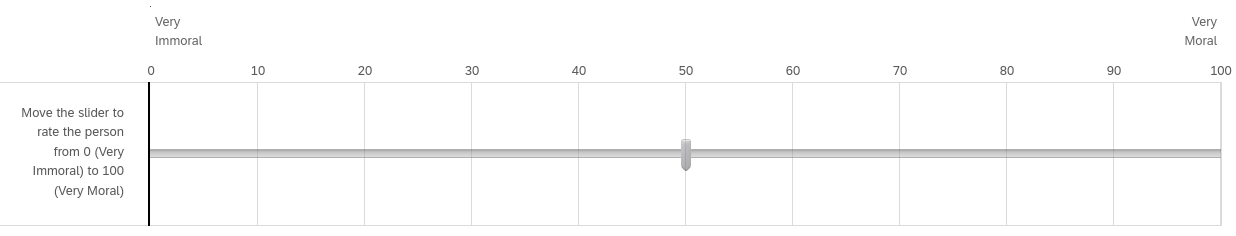
\includegraphics{../resources/images/mm1.png}
\newpage

\pagebreak

\section{Study 1 (bad): Supplementary Analyses}\label{study-1-bad-supplementary-analyses}

\subsection{Study 1: Combined Measure}\label{study-1-combined-measure}

We developed a combined moral perception measure by calculating the mean of the combined mean-centered scores for MPS-4 and MM-1, and mean-centering this result. Below we report the analyses for this combined measure.

The means and standard deviations for the combined measure for each scenario are as follows:
\emph{Sam},
\emph{M} = 0.02, \emph{SD} = 0.89,
\emph{Francis},
\emph{M} = 0.48, \emph{SD} = 1.00,
\emph{Alex},
\emph{M} = -0.21, \emph{SD} = 0.92,
\emph{Robin},
\emph{M} = -0.32, \emph{SD} = 0.94. There was significant variation depending on the description, \emph{F}(3,2255) = 269.01, \emph{p} \textless{} .001, partial \(\eta\)\textsuperscript{2} = 0.10. \emph{Francis} appeared to be rated as the most favorable, followed by \emph{Sam}, then \emph{Alex} and finally \emph{Robin} as the least favorable (all \emph{p}s \textless{} .001).

We conducted a linear-mixed-effects model to test if condition influenced moral perception. Our outcome measure was the combined moral perception measure, our predictor variable was condition; we allowed intercepts and the effect of condition to vary across participants, and scenario was also included in the model.
Overall, the model significantly predicted participants responses, and provided a better fit for the data than the baseline model, \(\chi\)\textsuperscript{2}(8) = 762.31, \emph{p} \textless{} .001. Condition significantly influenced responses to the MPS-4, \emph{F}(1, 799.66) = 57.93, \emph{p} \textless{} .001; and was a significant predictor in the model when controlling for scenario, \(b\) = -0.08, \emph{t}(2,501.32) = -3.42, \emph{p} \textless{} .001, with the non-diagnostic descriptions being rated as more moral than the diagnostic (morally relevant) descriptions of immoral characters Figure~\ref{fig:S1combinedconditionplot}.

\begin{figure}[!h]
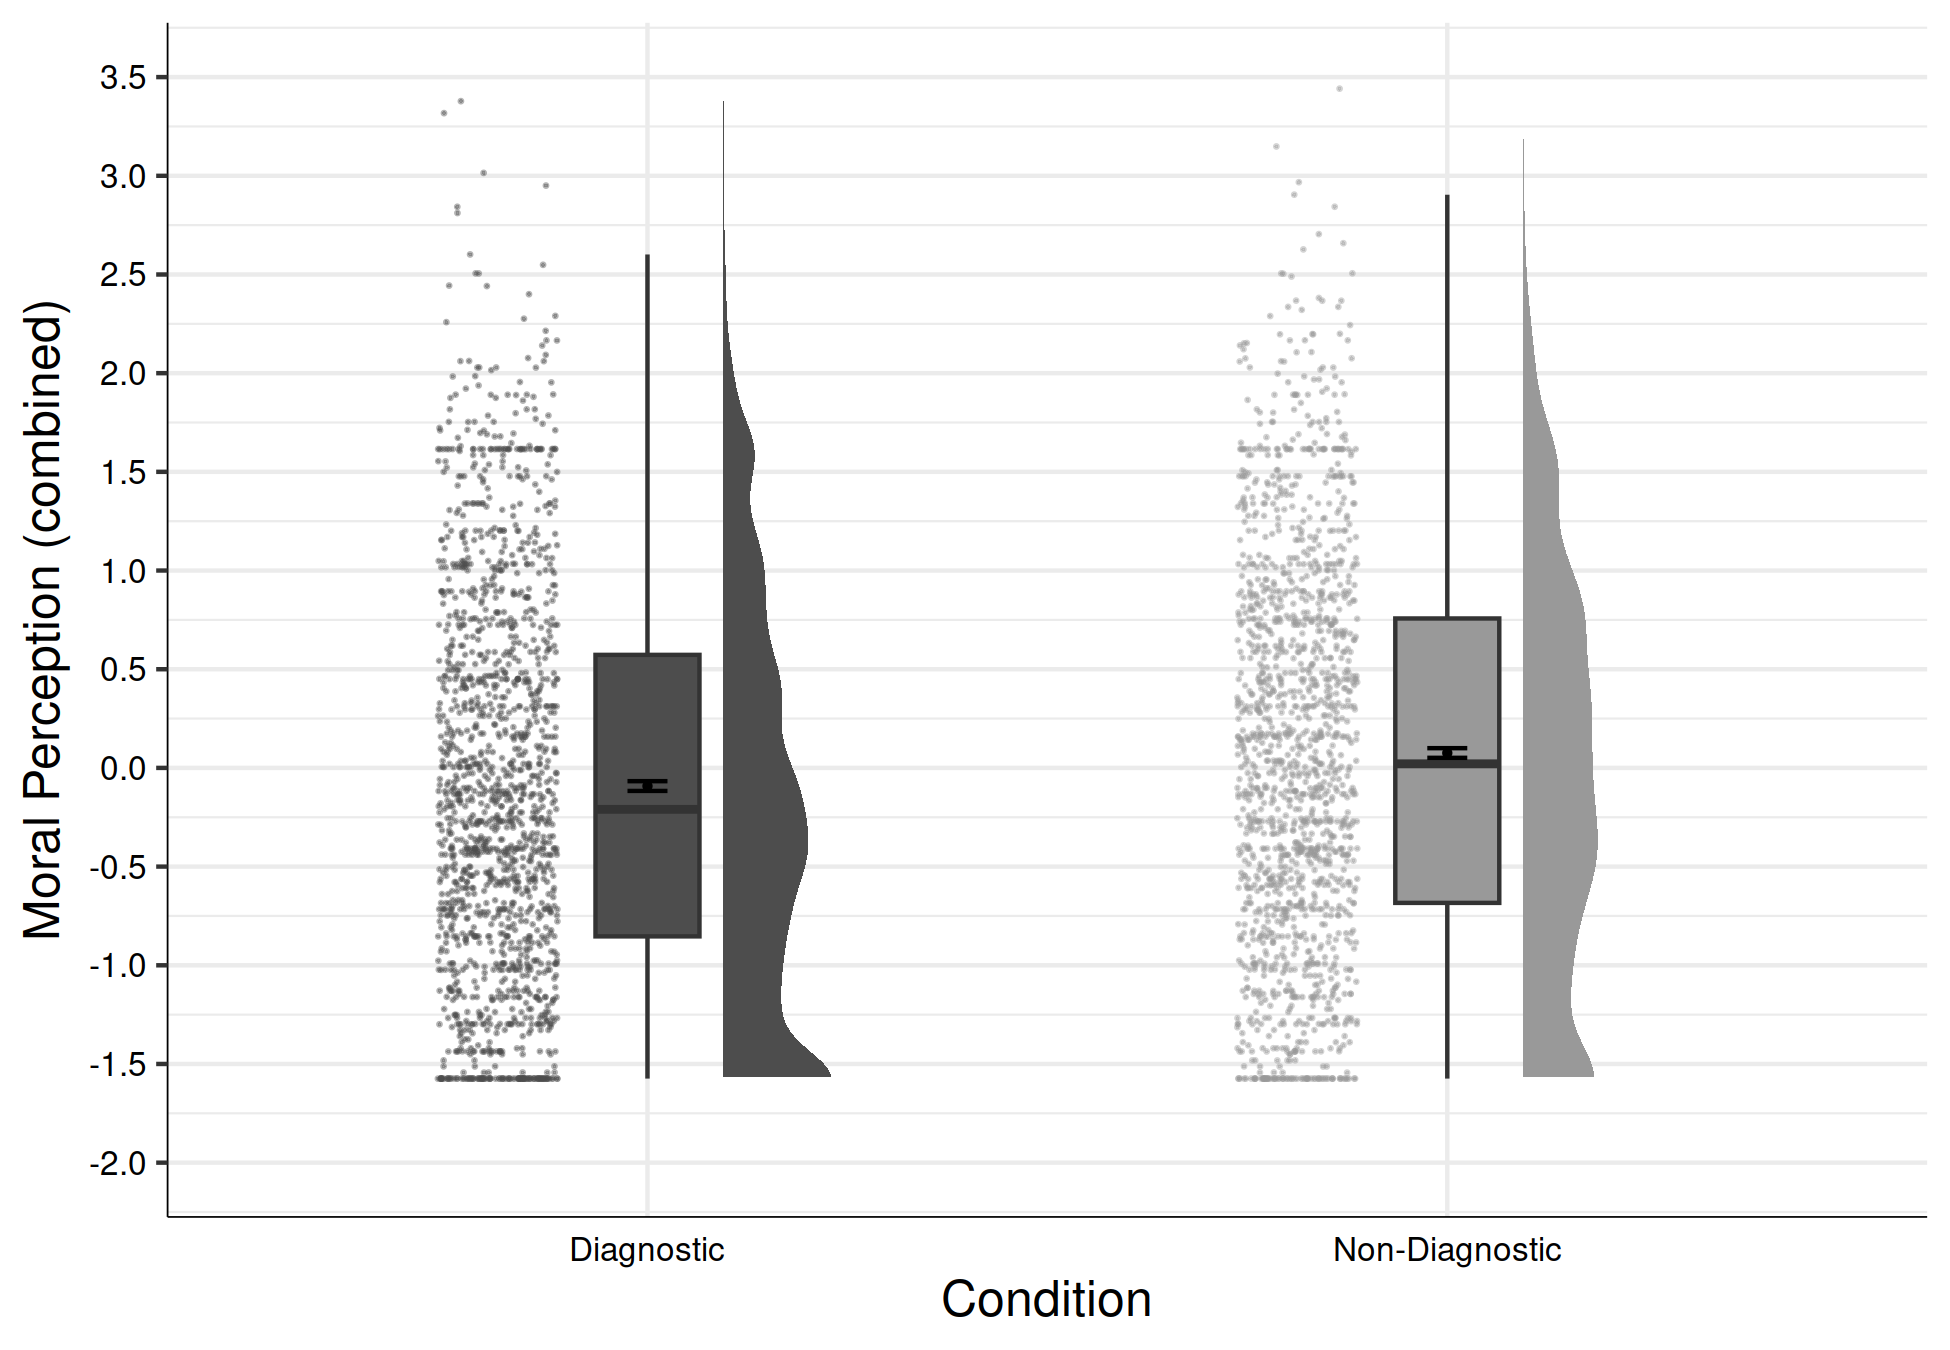
\includegraphics[width=\textwidth,]{Supplementary_files/figure-latex/S1combinedconditionplot-1} \caption{Study 1: Differences in combined measure depending on condition}\label{fig:S1combinedconditionplot}
\end{figure}

\newpage

\subsection{Study 1: Differences between the Descriptions}\label{study-1-differences-between-the-descriptions}

We additionally conducted separate analyses for each scenario individually (for each dependent measure MPS-4, MM-1 and the combined measure). The responses for each scenario across each measure depending on condition are displayed in Figure~\ref{fig:S1allscenariosPlot}.

\begin{figure}[!p]
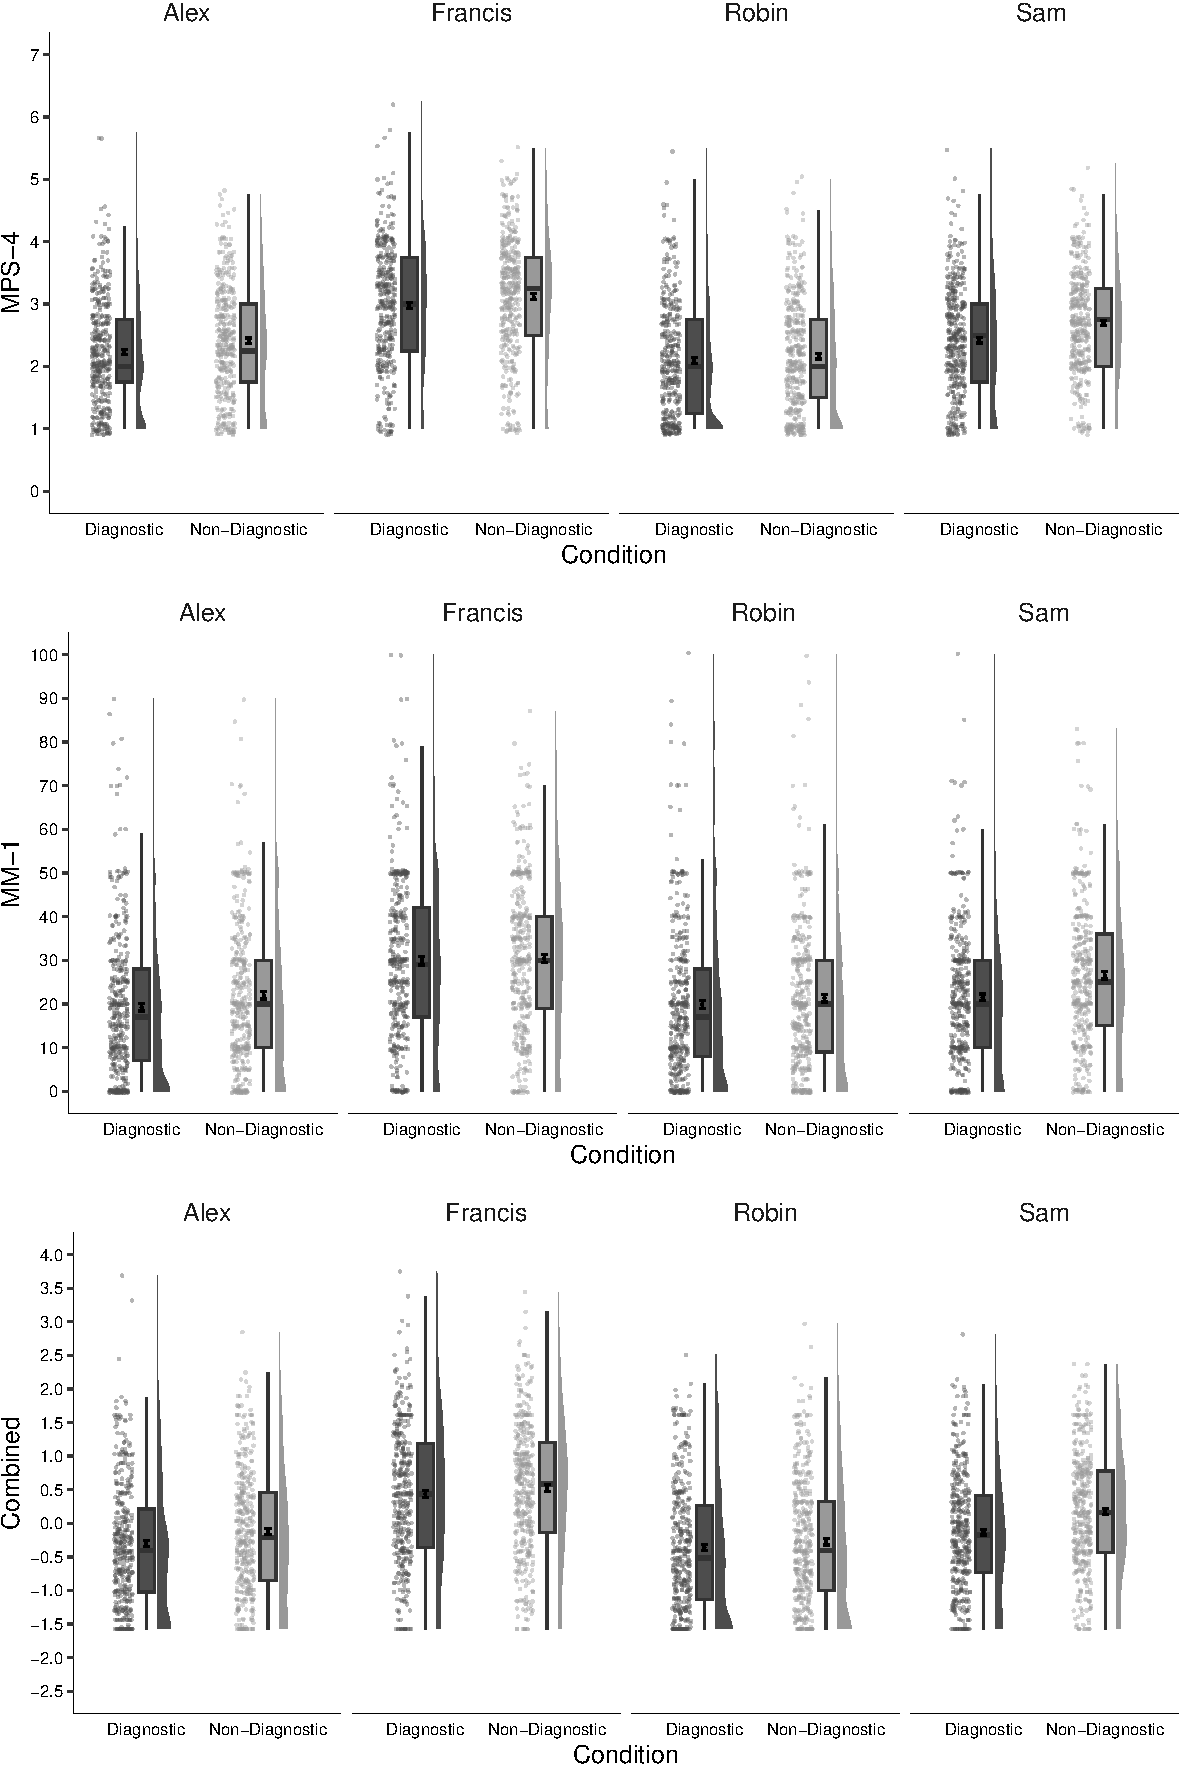
\includegraphics{Supplementary_files/figure-latex/S1allscenariosPlot-1} \caption{Study 1: Differences in moral perception for each description}\label{fig:S1allscenariosPlot}
\end{figure}

For \emph{Sam}, MPS-4 scores were significantly higher for the non-diagnostic condition (\emph{M} = 2.70, \emph{SD} = 0.82), than in the diagnostic condition (\emph{M} = 2.42, \emph{SD} = 0.87), \emph{t}(798.90) = -4.66, \emph{p} \textless{} .001, \emph{d} = 0.33; MM-1 ratings were higher in the non-diagnostic condition (\emph{M} = 26.55, \emph{SD} = 16.41), than in the diagnostic condition (\emph{M} = 21.50, \emph{SD} = 15.59), \emph{t}(787.84) = -4.45, \emph{p} \textless{} .001, \emph{d} = 0.32. For the combined measure ratings were also higher in the non-diagnostic condition (\emph{M} = 0.18, \emph{SD} = 0.88), than in the diagnostic condition (\emph{M} = -0.13, \emph{SD} = 0.88), \emph{t}(795.41) = -4.98, \emph{p} \textless{} .001, \emph{d} = 0.35.

For \emph{Robin}, MPS-4 scores were not significantly different for the non-diagnostic condition (\emph{M} = 2.16, \emph{SD} = 0.90), than in the diagnostic condition (\emph{M} = 2.09, \emph{SD} = 0.92), \emph{t}(793.94) = -1.09, \emph{p} = .275, \emph{d} = 0.08; MM-1 ratings were similar in the non-diagnostic condition (\emph{M} = 21.29, \emph{SD} = 16.94), and in the diagnostic condition (\emph{M} = 19.87, \emph{SD} = 17.17), \emph{t}(794.97) = -1.18, \emph{p} = .239, \emph{d} = 0.08. For the combined measure ratings were also similar in the non-diagnostic condition (\emph{M} = -0.28, \emph{SD} = 0.94), and in the diagnostic condition (\emph{M} = -0.36, \emph{SD} = 0.94), \emph{t}(796.03) = -1.24, \emph{p} = .217, \emph{d} = 0.09.

For \emph{Alex}, MPS-4 scores were significantly higher for the non-diagnostic condition (\emph{M} = 2.41, \emph{SD} = 0.88), than in the diagnostic condition (\emph{M} = 2.23, \emph{SD} = 0.86), \emph{t}(796.97) = -2.92, \emph{p} = .004, \emph{d} = 0.21; MM-1 ratings were higher in the non-diagnostic condition (\emph{M} = 21.93, \emph{SD} = 16.47), than in the diagnostic condition (\emph{M} = 19.20, \emph{SD} = 16.73), \emph{t}(798.89) = -2.33, \emph{p} = .020, \emph{d} = 0.16. For the combined measure ratings were also higher in the non-diagnostic condition (\emph{M} = -0.12, \emph{SD} = 0.92), than in the diagnostic condition (\emph{M} = -0.30, \emph{SD} = 0.92), \emph{t}(798.40) = -2.82, \emph{p} = .005, \emph{d} = 0.20.

For \emph{Francis}, MPS-4 scores were significantly higher for the non-diagnostic condition (\emph{M} = 3.12, \emph{SD} = 0.95), than in the diagnostic condition (\emph{M} = 2.98, \emph{SD} = 0.97), \emph{t}(796.12) = -1.99, \emph{p} = .047, \emph{d} = 0.14; MM-1 ratings were not significantly different in the non-diagnostic condition (\emph{M} = 30.38, \emph{SD} = 17.17), than in the diagnostic condition (\emph{M} = 29.84, \emph{SD} = 18.56), \emph{t}(788.61) = -0.43, \emph{p} = .668, \emph{d} = 0.03. For the combined measure ratings were also similar in the non-diagnostic condition (\emph{M} = 0.53, \emph{SD} = 0.98), and in the diagnostic condition (\emph{M} = 0.44, \emph{SD} = 1.02), \emph{t}(794.36) = -1.29, \emph{p} = .198, \emph{d} = 0.09.

\pagebreak

\section{Study 2 (good): Supplementary Analyses}\label{study-2-good-supplementary-analyses}

\subsection{Study 2: Combined Measure}\label{study-2-combined-measure}

Below we report the results for the combined measure of moral perception. We additionally report the effect of condition on responses to each description individually

The means and standard deviations for the combined measure for each scenario are as follows:
\emph{Sam},
\emph{M} = 0.07, \emph{SD} = 0.97,
\emph{Francis},
\emph{M} = -0.17, \emph{SD} = 1.06,
\emph{Alex},
\emph{M} = 0.09, \emph{SD} = 1.02,
\emph{Robin},
\emph{M} = 0.07, \emph{SD} = 0.96. There was significant variation depending on the description, \emph{F}(3,2335) = 48.01, \emph{p} \textless{} .001, partial \(\eta\)\textsuperscript{2} = 0.01. \emph{Francis} appeared to be rated as the less favorable than all other characters (all \emph{p}s \textless{} .001), there were no differences between \emph{Sam}, \emph{Robin}, and \emph{Alex} (all \emph{p}s \textgreater{} .05).

We conducted a linear-mixed-effects model to test if condition influenced moral perception. Our outcome measure was the combined moral perception measure, our predictor variable was condition; we allowed intercepts and the effect of condition to vary across participants, and scenario was also included in the model.
Overall, the model significantly predicted participants responses, and provided a better fit for the data than the baseline model, \(\chi\)\textsuperscript{2}(8) = 142.42, \emph{p} \textless{} .001. Condition did not influence moral perception, \emph{F}(1, 2,452.92) = 0.88, \emph{p} = .349; and was not a significant predictor in the model when controlling for scenario, \(b\) = -0.01, \emph{t}(2,613.53) = -0.42, \emph{p} = .673, see Figure~\ref{fig:S3combinedconditionplot}.

\begin{figure}[!h]
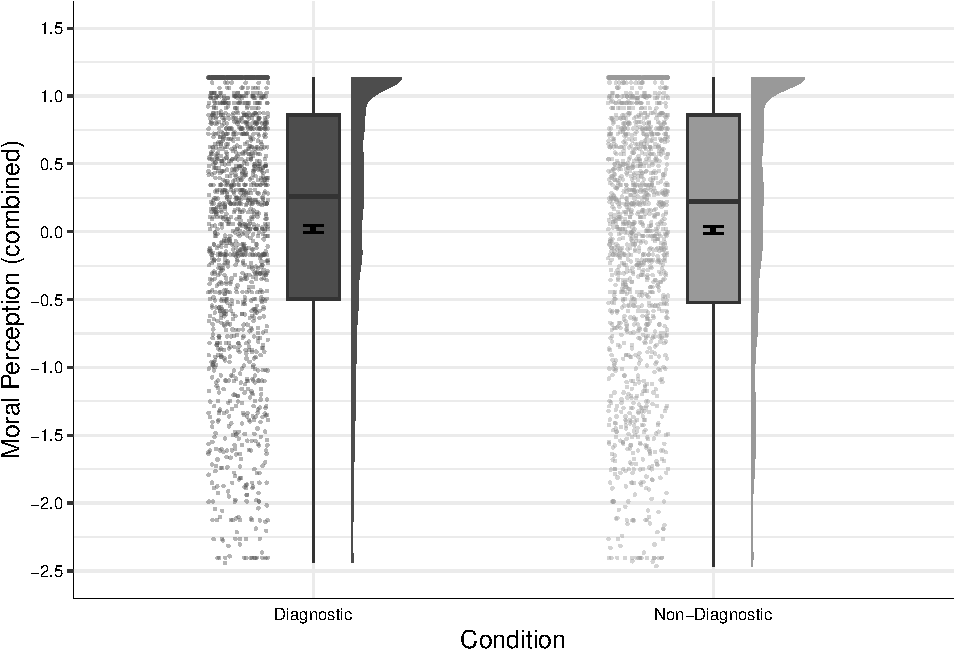
\includegraphics[width=\textwidth,]{Supplementary_files/figure-latex/S3combinedconditionplot-1} \caption{Study 2: Differences in combined measure depending on condition}\label{fig:S3combinedconditionplot}
\end{figure}

\newpage

\subsection{Study 2: Differences between the Descriptions}\label{study-2-differences-between-the-descriptions}

Below we provide analyses of the effect of condition on responses to each scenario individually. The responses for each scenario across each measure depending on condition are displayed in Figure~\ref{fig:S2allscenariosPlot}.

For \emph{Sam}, MPS-4 scores were not significantly different in the non-diagnostic condition (\emph{M} = 6.17, \emph{SD} = 0.89), than in the diagnostic condition (\emph{M} = 6.05, \emph{SD} = 1.06), \emph{t}(680.49) = -1.71, \emph{p} = .088, \emph{d} = 0.12; MM-1 ratings were similar in the non-diagnostic condition (\emph{M} = 84.90, \emph{SD} = 14.26), and in the diagnostic condition (\emph{M} = 84.20, \emph{SD} = 14.76), \emph{t}(744.17) = -0.69, \emph{p} = .490, \emph{d} = 0.05. For the combined measure ratings were also similar in the non-diagnostic condition (\emph{M} = 0.11, \emph{SD} = 0.93), and in the diagnostic condition (\emph{M} = 0.02, \emph{SD} = 1.03), \emph{t}(717.94) = -1.33, \emph{p} = .183, \emph{d} = 0.10.

\newpage

\begin{figure}[!p]
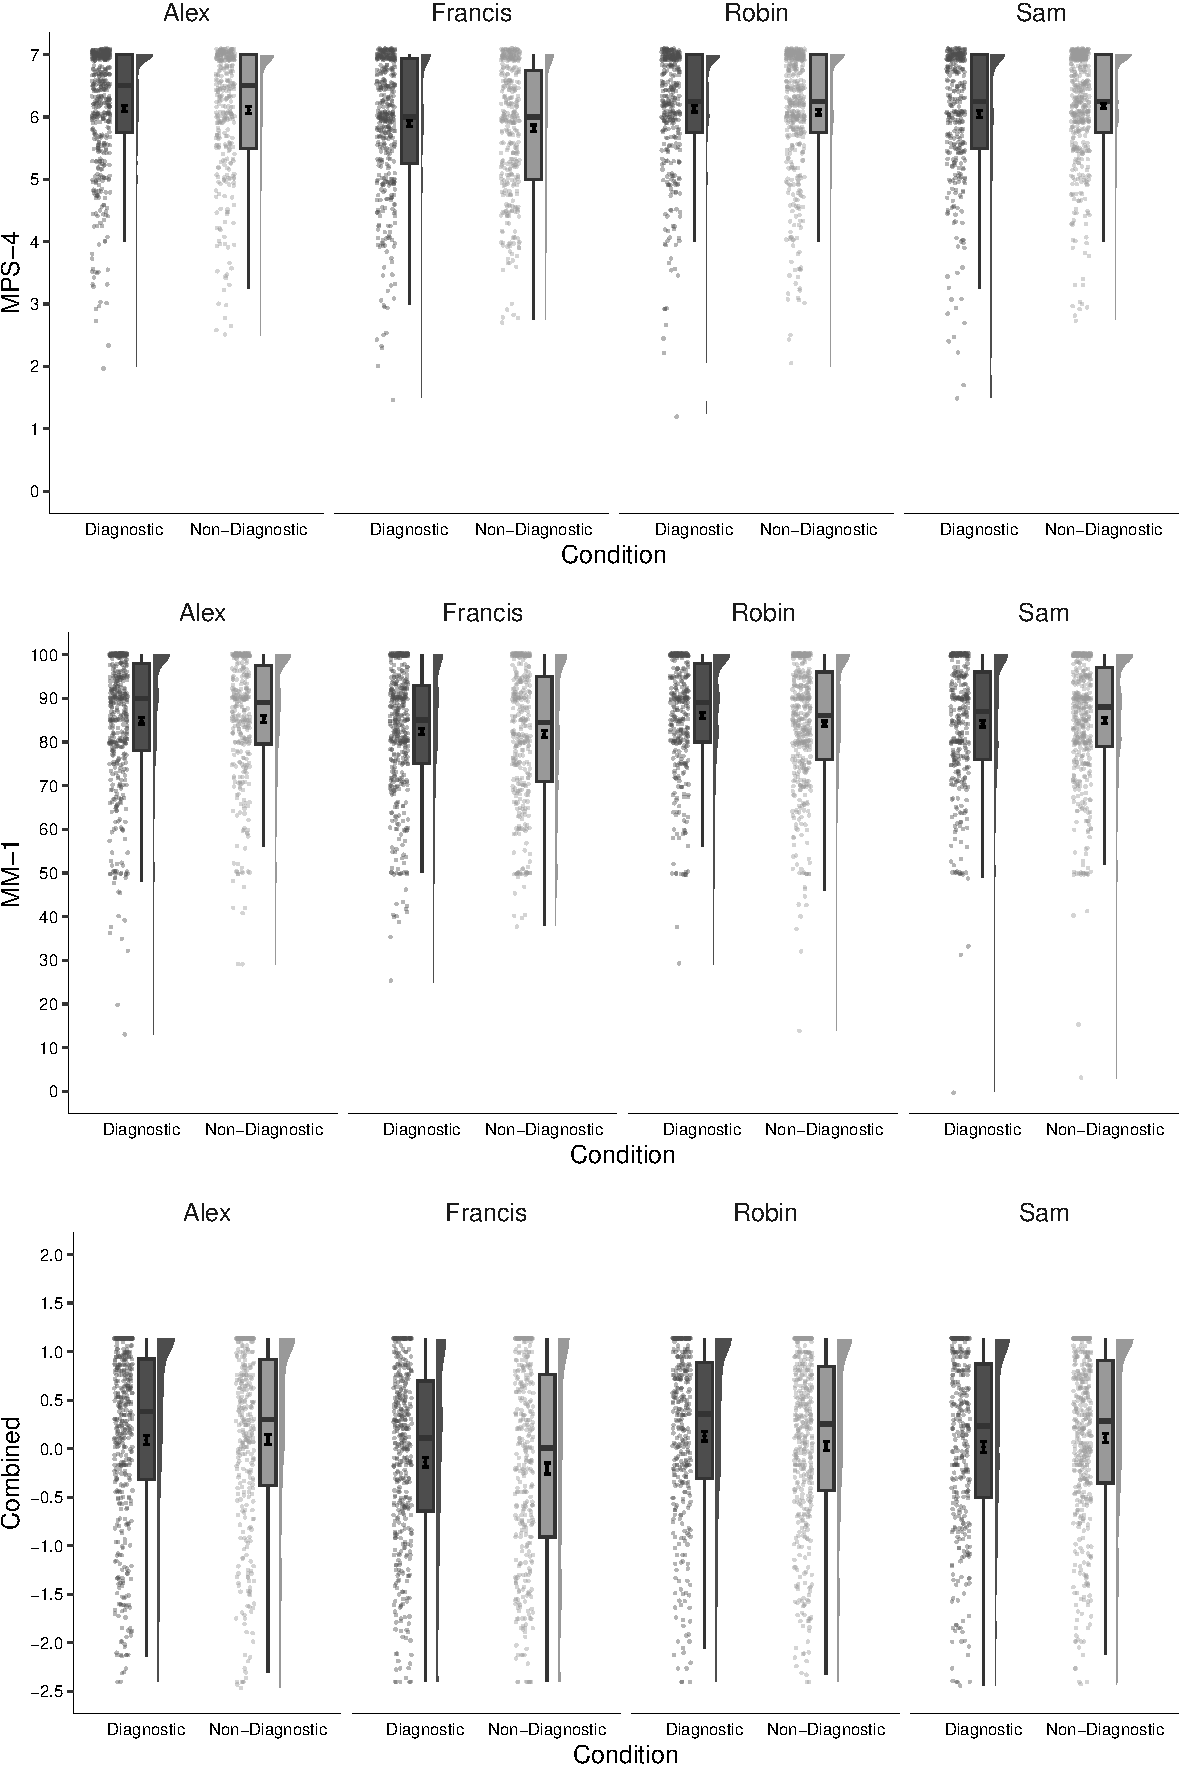
\includegraphics{Supplementary_files/figure-latex/S2allscenariosPlot-1} \caption{Study 2: Differences in moral perception for each description}\label{fig:S2allscenariosPlot}
\end{figure}

For \emph{Robin}, MPS-4 scores were not significantly different for the non-diagnostic condition (\emph{M} = 6.08, \emph{SD} = 1.00), than in the diagnostic condition (\emph{M} = 6.13, \emph{SD} = 0.98), \emph{t}(784.04) = 0.73, \emph{p} = .463, \emph{d} = 0.05; MM-1 ratings were similar in the non-diagnostic condition (\emph{M} = 84.12, \emph{SD} = 14.37), and in the diagnostic condition (\emph{M} = 85.98, \emph{SD} = 13.32), \emph{t}(800.09) = 1.92, \emph{p} = .055, \emph{d} = 0.13. For the combined measure ratings were also similar in the non-diagnostic condition (\emph{M} = 0.03, \emph{SD} = 0.98), and in the diagnostic condition (\emph{M} = 0.13, \emph{SD} = 0.95), \emph{t}(788.76) = 1.46, \emph{p} = .145, \emph{d} = 0.10.

For \emph{Alex}, MPS-4 scores were not significantly different for the non-diagnostic condition (\emph{M} = 6.11, \emph{SD} = 1.00), than in the diagnostic condition (\emph{M} = 6.14, \emph{SD} = 0.99), \emph{t}(737.60) = 0.32, \emph{p} = .746, \emph{d} = 0.02; MM-1 ratings were similar in the non-diagnostic condition (\emph{M} = 85.28, \emph{SD} = 14.31), and in the diagnostic condition (\emph{M} = 84.83, \emph{SD} = 15.51), \emph{t}(776.47) = -0.43, \emph{p} = .668, \emph{d} = 0.03. For the combined measure ratings were also similar in the non-diagnostic condition (\emph{M} = 0.09, \emph{SD} = 0.98), and in the diagnostic condition (\emph{M} = 0.09, \emph{SD} = 1.04), \emph{t}(767.89) = -0.06, \emph{p} = .952, \emph{d} = 0.00.

For \emph{Francis}, MPS-4 scores were not significantly different for the non-diagnostic condition (\emph{M} = 5.82, \emph{SD} = 1.05), than in the diagnostic condition (\emph{M} = 5.90, \emph{SD} = 1.08), \emph{t}(794.94) = 1.06, \emph{p} = .290, \emph{d} = 0.07; MM-1 ratings were not significantly different in the non-diagnostic condition (\emph{M} = 81.74, \emph{SD} = 15.67), than in the diagnostic condition (\emph{M} = 82.31, \emph{SD} = 14.90), \emph{t}(771.23) = 0.54, \emph{p} = .591, \emph{d} = 0.04. For the combined measure ratings were also similar in the non-diagnostic condition (\emph{M} = -0.20, \emph{SD} = 1.08), and in the diagnostic condition (\emph{M} = -0.14, \emph{SD} = 1.04), \emph{t}(777.51) = 0.88, \emph{p} = .379, \emph{d} = 0.06.

\pagebreak

\section{Study 3 (bad and good): Supplementary Analyses}\label{study-3-bad-and-good-supplementary-analyses}

\subsection{Study 3: Combined Measure}\label{study-3-combined-measure}

Below we report the results for the combined measure of moral perception from both DVs. We additionally report the effect of condition on responses to each description individually

The means and standard deviations for the combined measure for each scenario are as follows:
\emph{Sam},
\emph{M} = 0.93, \emph{SD} = 0.39,
\emph{Francis},
\emph{M} = -1.17, \emph{SD} = 0.42,
\emph{Alex},
\emph{M} = -1.08, \emph{SD} = 0.46,
\emph{Robin},
\emph{M} = 0.99, \emph{SD} = 0.36. There was significant variation depending on the description, \emph{F}(2,1403) = 6,772.79, \emph{p} \textless{} .001, partial \(\eta\)\textsuperscript{2} = 0.87. Both the \emph{good} characters (\emph{Robin} and \emph{Sam}) were rated significantly more favorably than both the \emph{bad} characters (\emph{Alex} and \emph{Francis}; all \emph{p}s \textless{} .001). For the \emph{good} characters, \emph{Robin} was rated higher than \emph{Sam} (\emph{p} \textless{} .001), and for the \emph{bad} characters \emph{Francis} was rated more negatively than \emph{Alex} (\emph{p} \textless{} .001).

We conducted a linear-mixed-effects model to test if our predictors influenced responses on the combined moral perception measure. Our outcome measure was the combined moral perception measure, our predictor variables were condition and valence; we allowed intercepts and the effects of condition and valence to vary across participants.
Overall, the model significantly predicted participants responses, and provided a better fit for the data than the baseline model,
\(\chi\)\textsuperscript{2}(5) = 1,796.22, \emph{p} \textless{} .001.
Condition significantly influenced responses to the combined moral perception measure,
\emph{F}(1, 828) = 47.25, \emph{p} \textless{} .001
and was a significant predictor in the model when controlling for scenario, \(b\) = -0.07, \emph{t}(827.54) = -6.87, \emph{p} \textless{} .001;
valence significantly predicted responses,
\emph{F}(1, 826) = 1,476.93, \emph{p} \textless{} .001;
and there was also a significant condition \(\times\) valence interaction,
\emph{F}(1, 821) = 4.23, \emph{p} = .040, see Figure~\ref{fig:S3combinedplot}.

For the \emph{bad} characters, we conducted a linear-mixed-effects model to test if condition influenced responses to the combined measure. Our outcome measure was the combined moral perception measure, our predictor variable was condition; we allowed intercepts and the effect of condition to vary across participants. Overall, the model significantly predicted participants responses, and provided a better fit for the data than the baseline model, \(\chi\)\textsuperscript{2}(3) = 74.54, \emph{p} \textless{} .001. Condition significantly influenced MPS-4 responses \emph{F}(1, 820.39) = 37.63, \emph{p} \textless{} .001, and was a significant predictor in the model \(b\) = -0.04, \emph{t}(820.39) = -6.13, \emph{p} \textless{} .001.

For the \emph{good} characters, we conducted a linear-mixed-effects model to test if condition influenced responses to the combined measure. Our outcome measure was the combined moral perception measure, our predictor variable was condition; we allowed intercepts and the effect of condition to vary across participants. Overall, the model significantly predicted participants responses, and provided a better fit for the data than the baseline model, \(\chi\)\textsuperscript{2}(3) = 45.20, \emph{p} \textless{} .001. Condition significantly influenced MPS-4 responses \emph{F}(1, 826.21) = 15.67, \emph{p} \textless{} .001, and was a significant predictor in the model \(b\) = 0.02, \emph{t}(826.21) = 3.96, \emph{p} \textless{} .001.

\begin{figure}[!h]
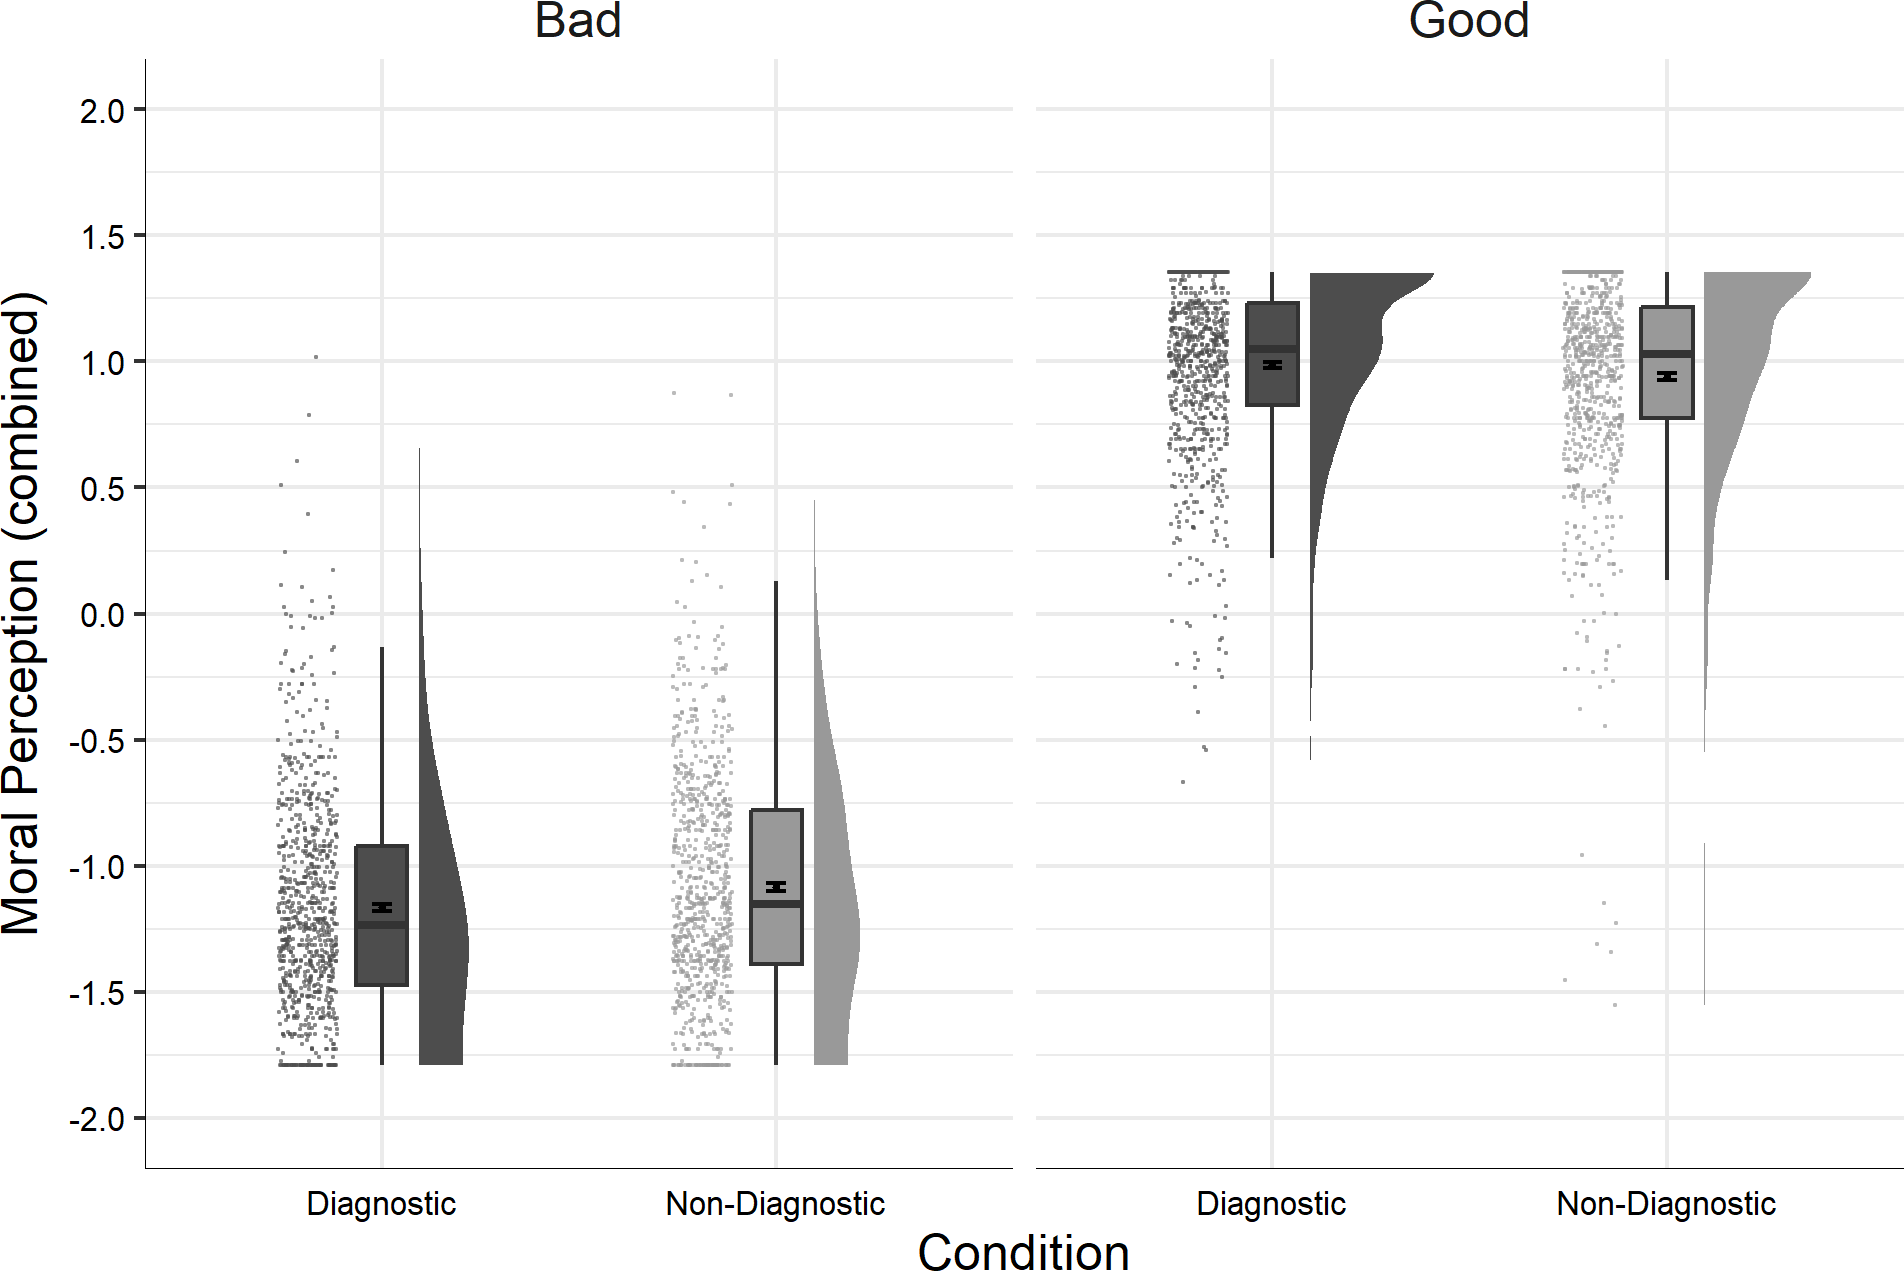
\includegraphics[width=\textwidth,]{Supplementary_files/figure-latex/S3combinedplot-1} \caption{Study 3: Differences in the combined measure depending on condition}\label{fig:S3combinedplot}
\end{figure}

\newpage

\subsection{Study 3: Differences between the descriptions}\label{study-3-differences-between-the-descriptions}

Again, we conducted separate analyses to investigate of condition on responses to each scenario individually. The responses for each scenario across each measure depending on condition are displayed in Figure~\ref{fig:S3allscenariosPlot}.

For \emph{Sam}, MPS-4 scores were not significantly lower in the non-diagnostic condition (\emph{M} = 6.15, \emph{SD} = 0.86), than in the diagnostic condition (\emph{M} = 6.25, \emph{SD} = 0.76), \emph{t}(812.83) = 1.68, \emph{p} = .094, \emph{d} = 0.12; Similarly, MM-1 ratings were similar in the non-diagnostic condition (\emph{M} = 85.49, \emph{SD} = 14.10), in the diagnostic condition (\emph{M} = 87.18, \emph{SD} = 13.21), \emph{t}(821.76) = 1.78, \emph{p} = .075, \emph{d} = 0.12. For the combined measure ratings was also no significant difference between the non-diagnostic condition (\emph{M} = 0.90, \emph{SD} = 0.42), and the diagnostic condition (\emph{M} = 0.96, \emph{SD} = 0.37), \emph{t}(811.12) = 1.88, \emph{p} = .060, \emph{d} = 0.13.

For \emph{Robin}, MPS-4 scores were not significantly different for the non-diagnostic condition (\emph{M} = 6.28, \emph{SD} = 0.80), than in the diagnostic condition (\emph{M} = 6.36, \emph{SD} = 0.71), \emph{t}(809.44) = 1.60, \emph{p} = .111, \emph{d} = 0.11; MM-1 ratings were similar in the non-diagnostic condition (\emph{M} = 87.84, \emph{SD} = 13.49), and in the diagnostic condition (\emph{M} = 89.02, \emph{SD} = 10.30), \emph{t}(765.30) = 1.42, \emph{p} = .156, \emph{d} = 0.10. For the combined measure ratings were also similar in the non-diagnostic condition (\emph{M} = 0.97, \emph{SD} = 0.39), than in the diagnostic condition (\emph{M} = 1.01, \emph{SD} = 0.32), \emph{t}(784.03) = 1.63, \emph{p} = .103, \emph{d} = 0.11.

For \emph{Alex}, MPS-4 scores were significantly higher for the non-diagnostic condition (\emph{M} = 2.41, \emph{SD} = 0.88), than in the diagnostic condition (\emph{M} = 2.24, \emph{SD} = 0.90), \emph{t}(830.38) = -2.69, \emph{p} = .007, \emph{d} = 0.19; MM-1 ratings were similar in the non-diagnostic condition (\emph{M} = 23.53, \emph{SD} = 16.61), and in the diagnostic condition (\emph{M} = 22.62, \emph{SD} = 18.34), \emph{t}(828.19) = -0.75, \emph{p} = .454, \emph{d} = 0.05. For the combined measure ratings were also similar in the non-diagnostic condition (\emph{M} = -1.05, \emph{SD} = 0.45), and in the diagnostic condition (\emph{M} = -1.11, \emph{SD} = 0.47), \emph{t}(830.90) = -1.77, \emph{p} = .077, \emph{d} = 0.12.

For \emph{Francis}, MPS-4 scores were significantly higher for the non-diagnostic condition (\emph{M} = 2.26, \emph{SD} = 0.85), than in the diagnostic condition (\emph{M} = 2.05, \emph{SD} = 0.70), \emph{t}(802.80) = -3.96, \emph{p} \textless{} .001, \emph{d} = 0.27; MM-1 ratings were significantly higher in the non-diagnostic condition (\emph{M} = 22.01, \emph{SD} = 17.84), than in the diagnostic condition (\emph{M} = 18.45, \emph{SD} = 15.76), \emph{t}(817.94) = -3.05, \emph{p} = .002, \emph{d} = 0.21. For the combined measure ratings were also significantly higher in the non-diagnostic condition (\emph{M} = -1.11, \emph{SD} = 0.46), than in the diagnostic condition (\emph{M} = -1.23, \emph{SD} = 0.38), \emph{t}(808.55) = -3.85, \emph{p} \textless{} .001, \emph{d} = 0.27.

\begin{figure}[!p]
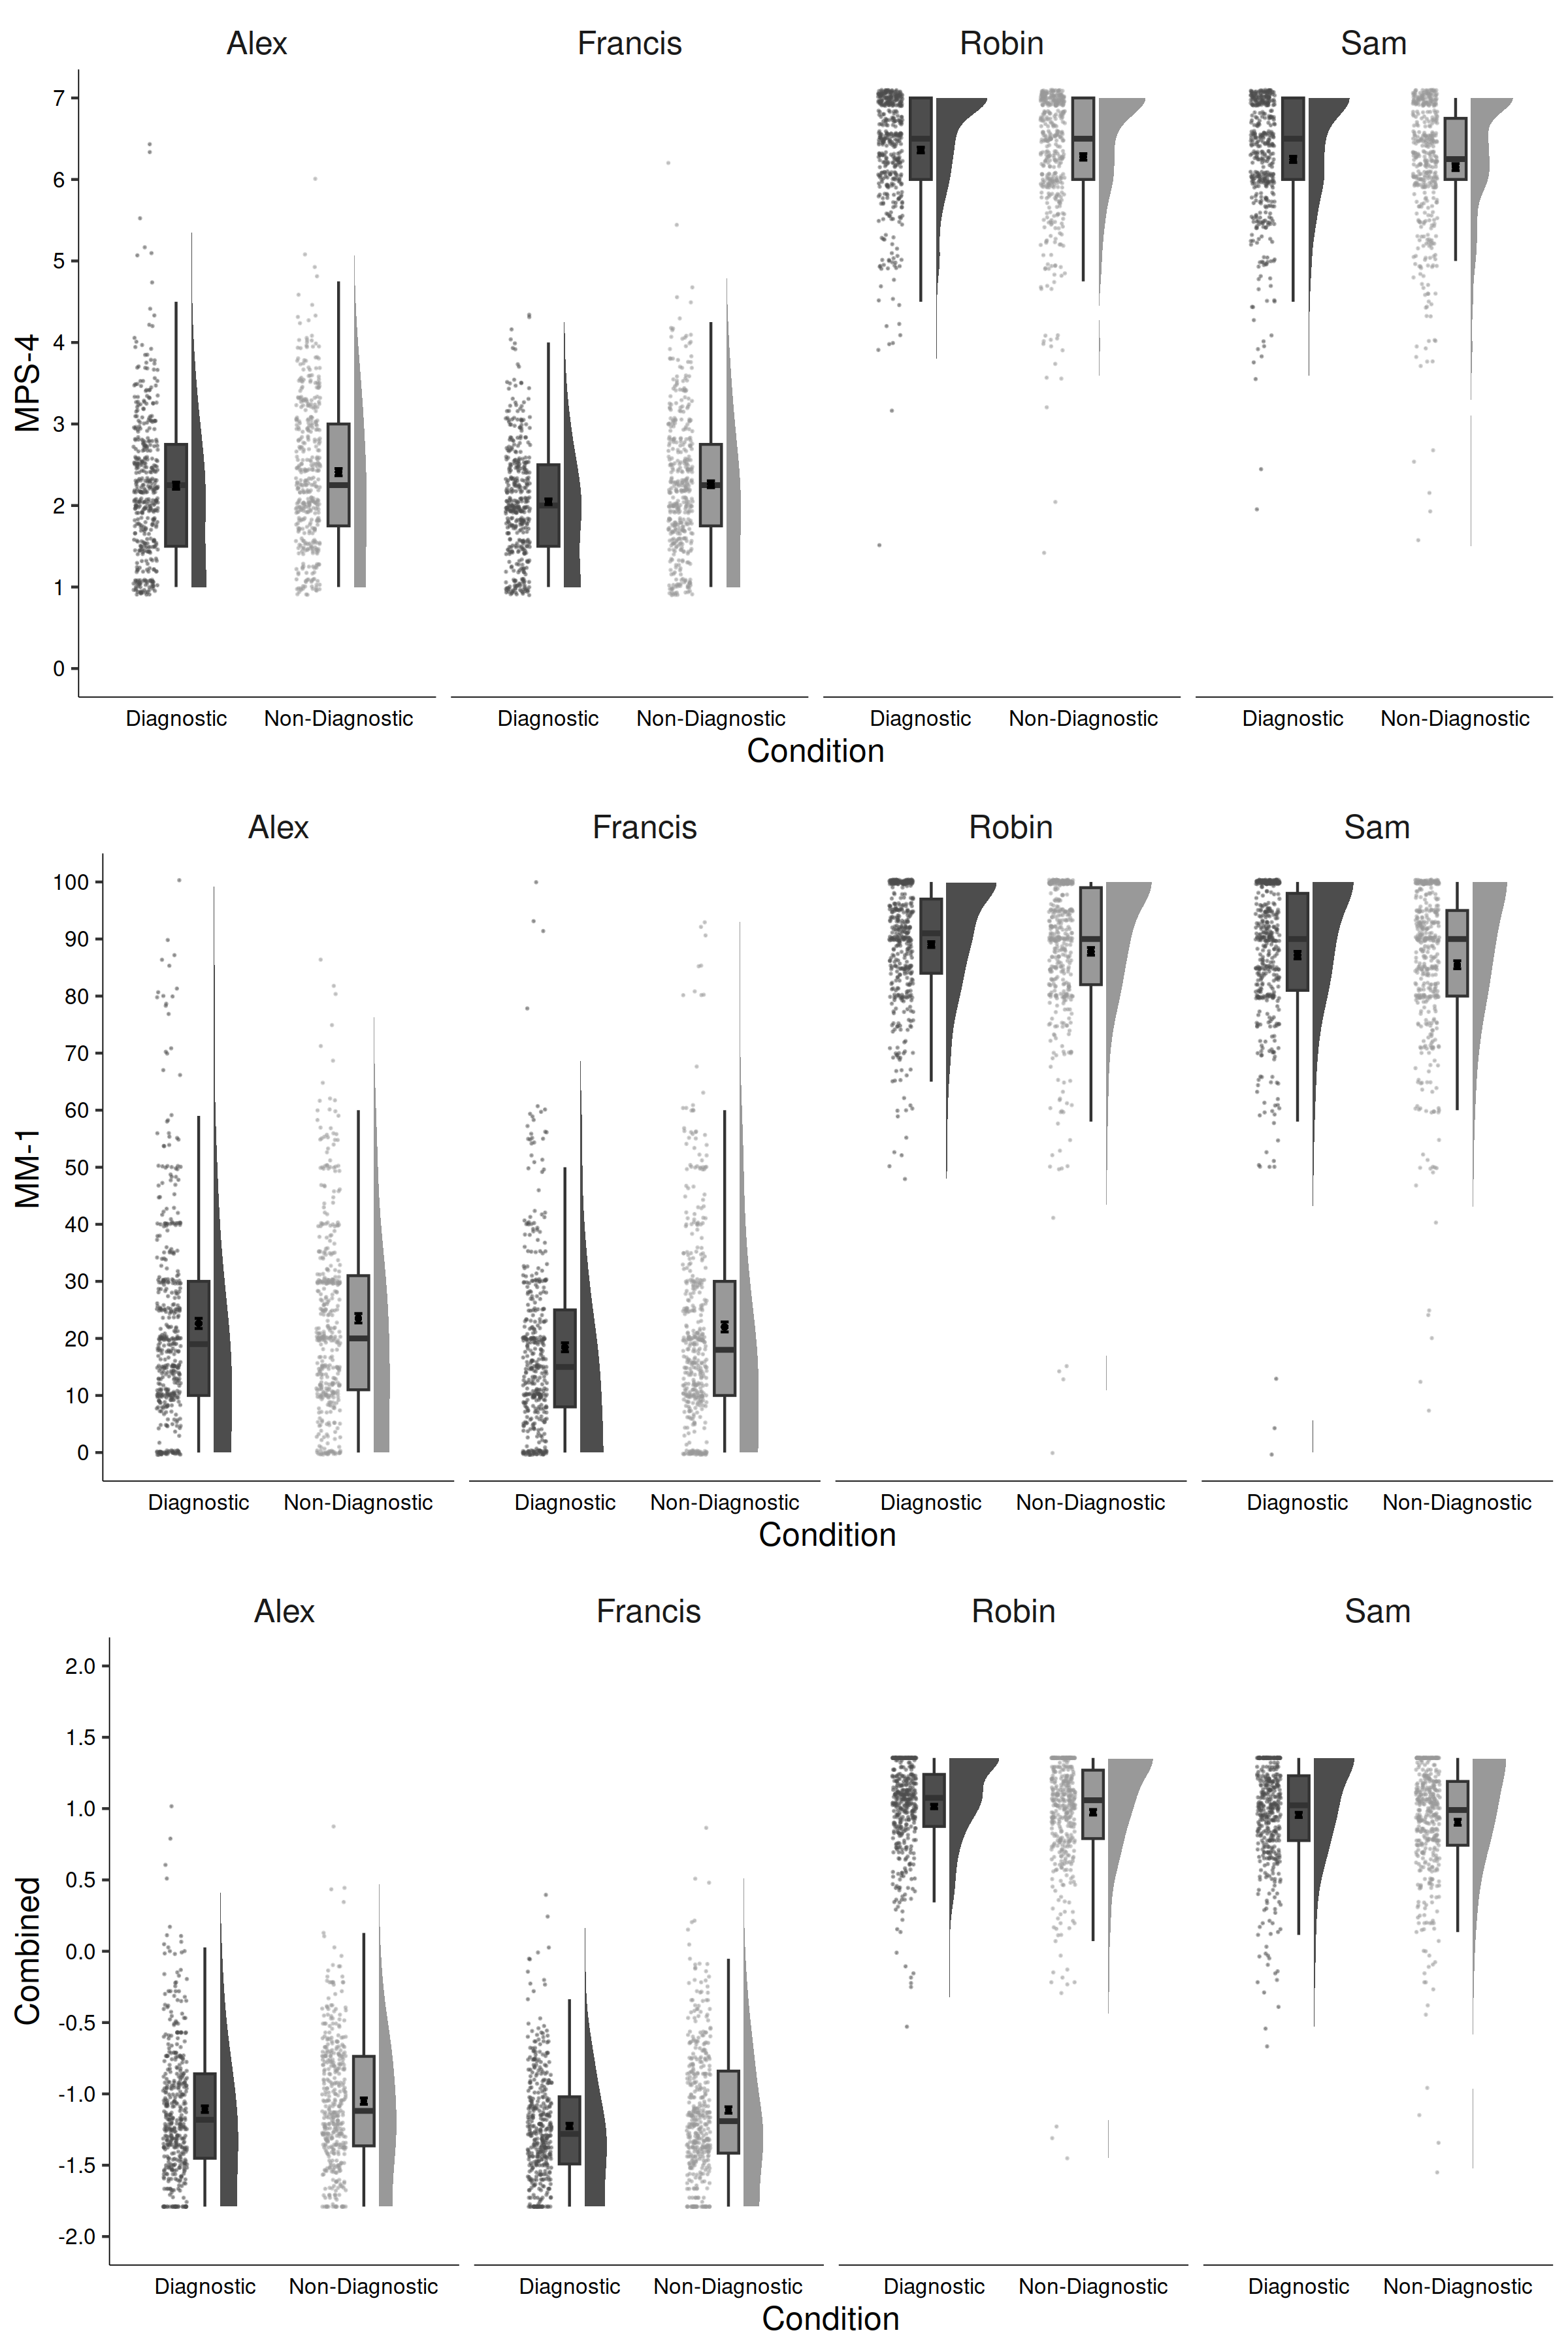
\includegraphics{Supplementary_files/figure-latex/S3allscenariosPlot-1} \caption{Study 3: Differences in moral perception for each description}\label{fig:S3allscenariosPlot}
\end{figure}

\pagebreak

\section{Pilot Study 1}\label{pilot-study-1}

The aim of this pilot study was to develop and test materials that could be used to study the dilution effect for moral characters. We developed diagnostic and non-diagnostic character descriptions. We hypothesized that moral evaluations of the diagnostic descriptions would be more severe (more immoral) than for the non-diagnostic descriptions.

\subsection{Pilot Study 1: Method}\label{pilot-study-1-method}

\subsubsection{Pilot 1: Participants and design}\label{pilot-1-participants-and-design}

The pilot study was a within-subjects design. The independent variable was description type with two levels, \emph{diagnostic} and \emph{non-diagnostic}. We used two dependent variables. The first dependent variable was the four item moral perception scale (MPS-4), participants rated the characters on four dimensions using 7-point bipolar scales. The dimensions and scale endpoints were: Bad-Good, Immoral-Moral, Violent-Peaceful, Merciless-Empathetic, this showed excellent reliability, \(\alpha\) = 0.93. The second dependent variable was a single item moral perception measure (MM-1) which consisted of a 100-point slider ranging from 0 = \emph{Very Immoral} to 100 = \emph{Very Moral}. Both dependent variables were taken from Walker et al. (2021).

A total sample of 235 (89 female, 142 male, 1 non-binary, 1 prefer not to say; \emph{M}\textsubscript{age} = 36.45, min = 20, max = 72, \emph{SD} = 10.23) started the survey. Participants were recruited from MTurk.

We removed participants who failed both manipulation checks (\emph{n} = 23), leaving a total sample of 212 participants (80 female, 128 male, 1 non-binary, 1 prefer not to say; \emph{M}\textsubscript{age} = 36.63, min = 20, max = 72, \emph{SD} = 10.34).

\subsubsection{Pilot 1: Procedure and materials}\label{pilot-1-procedure-and-materials}

Data were collected using an online questionnaire presented with Qualtrics (www.qualtrics.com). Participants were presented with descriptions of six characters.

Moral character descriptions were developed by combining descriptions relating to three different moral foundations. These descriptions were adapted from the items of the extended character morality questionnaire (Grizzard et al., 2020), and read as follows:

\begin{enumerate}
\def\labelenumi{(\roman{enumi})}
\tightlist
\item
  \emph{Imagine a person named Sam. Throughout their life they have been known to be cruel, act unfairly, and to betray their own group};
\item
  \emph{Imagine a person named Robin. Throughout their life they have been known to physically hurt others, treat some people differently to others, and show lack of loyalty};
\item
  \emph{Imagine a person named Francis. Throughout their life they have been known to violate the standards of purity and decency, show lack of respect for authority, and treat people unequally}
\item
  \emph{Imagine a person named Alex. Throughout their life they have been known to cause others to suffer emotionally, to deny others their rights, and to cause chaos or disorder}.
\end{enumerate}

We developed neutral descriptions that included information relating to physical appearance/attributes, hobbies/activities, and family information that read as follows:

\begin{enumerate}
\def\labelenumi{(\roman{enumi})}
\tightlist
\item
  \emph{Imagine a person named Jackie. They have red hair, play tennis four times a month, and have one older sibling and one younger sibling};
\item
  \emph{Imagine a person named Charlie. They are left-handed, drink tea in the morning, and have two older siblings and one younger sibling}.
\end{enumerate}

Character descriptions did not specify the gender of the charcters, and all characters had names that could be either male or female (Sam, Robin, Francis, Alex, Jackie, Charlie). All participants read six descriptions, four moral descriptions and two neutral. Pilot Study 1 was pre-registered at \color{blue}\url{https://aspredicted.org/3VK_8FD}\color{black}.

\subsection{Pilot 1: Results}\label{pilot-1-results}

\subsubsection{Pilot 1: Main Measures}\label{pilot-1-main-measures}

The means and standard deviations for MPS-4 for each scenario are as follows:
\emph{Sam} (diagnostic),
\emph{M}\textsubscript{MPS-4} = 4.35, \emph{SD}\textsubscript{MPS-4} = 1.90,
\emph{Francis} (diagnostic),
\emph{M}\textsubscript{MPS-4} = 4.46, \emph{SD}\textsubscript{MPS-4} = 1.73,
\emph{Alex} (diagnostic),
\emph{M}\textsubscript{MPS-4} = 4.44, \emph{SD}\textsubscript{MPS-4} = 1.79,
\emph{Robin} (diagnostic),
\emph{M}\textsubscript{MPS-4} = 4.35, \emph{SD}\textsubscript{MPS-4} = 1.96,
\emph{Jackie} (non-diagnostic),
\emph{M}\textsubscript{MPS-4} = 5.40, \emph{SD}\textsubscript{MPS-4} = 1.01,
\emph{Charlie} (non-diagnostic),
\emph{M}\textsubscript{MPS-4} = 5.38, \emph{SD}\textsubscript{MPS-4} = 1.01. For the diagnostic descriptions, there was no significant variation depending on the description, \emph{F}(3,600) = 1.58, \emph{p} = .194, partial \(\eta\)\textsuperscript{2} = 0.00. For the non-diagnostic descriptions there was no significant difference in ratings depending on description, \emph{t}(211) = -0.67, \emph{p} = .506, \emph{d} = 0.05.

The means and standard deviations for MM-1 for each scenario are as follows:
\emph{Sam} (diagnostic),
\emph{M}\textsubscript{MM-1} = 55.67, \emph{SD}\textsubscript{MM-1} = 30.47;
\emph{Francis} (diagnostic),
\emph{M}\textsubscript{MM-1} = 58.22, \emph{SD}\textsubscript{MM-1} = 28.61;
\emph{Alex} (diagnostic),
\emph{M}\textsubscript{MM-1} = 56.80, \emph{SD}\textsubscript{MM-1} = 29.45;
\emph{Robin} (diagnostic),
\emph{M}\textsubscript{MM-1} = 55.49, \emph{SD}\textsubscript{MM-1} = 31.38;
\emph{Jackie} (non-diagnostic),
\emph{M}\textsubscript{MM-1} = 73.00, \emph{SD}\textsubscript{MM-1} = 14.72;
\emph{Charlie} (non-diagnostic),
\emph{M}\textsubscript{MM-1} = 72.94, \emph{SD}\textsubscript{MM-1} = 14.79. For the diagnostic descriptions, we observed significant variation depending on the description, \emph{F}(3,608) = 3.01, \emph{p} = .032, partial \(\eta\)\textsuperscript{2} = 0.001. When correcting for multiple comparisons, pairwise comparisons did not reveal significant differences between descriptions. We note that without correction, \emph{Francis} appeared to be rated as more moral than both \emph{Robin} (\emph{p} = .012), and \emph{Sam} (\emph{p} = .009). For the non-diagnostic descriptions there was no significant difference in ratings depending on description, \emph{t}(211) = -0.09, \emph{p} = .929, \emph{d} = 0.01.

We conducted a linear-mixed-effects model to test if condition influenced MPS-4 responses. Our outcome measure was MPS-4, our predictor variable was condition; we allowed intercepts and the effect of condition to vary across participants.
Overall, the model significantly predicted participants responses, and provided a better fit for the data than the baseline model, \(\chi\)\textsuperscript{2}(2) = 860.16, \emph{p} \textless{} .001. Condition was a significant predictor in the model \(b\) = -0.49, \emph{t}(211.05) = -8.54, \emph{p} \textless{} .001, with the non-diagnostic descriptions being rated as more moral than the diagnostic descriptions of immoral characters Figure~\ref{fig:pilot1bothconditionplot}.

\begin{figure}[!h]
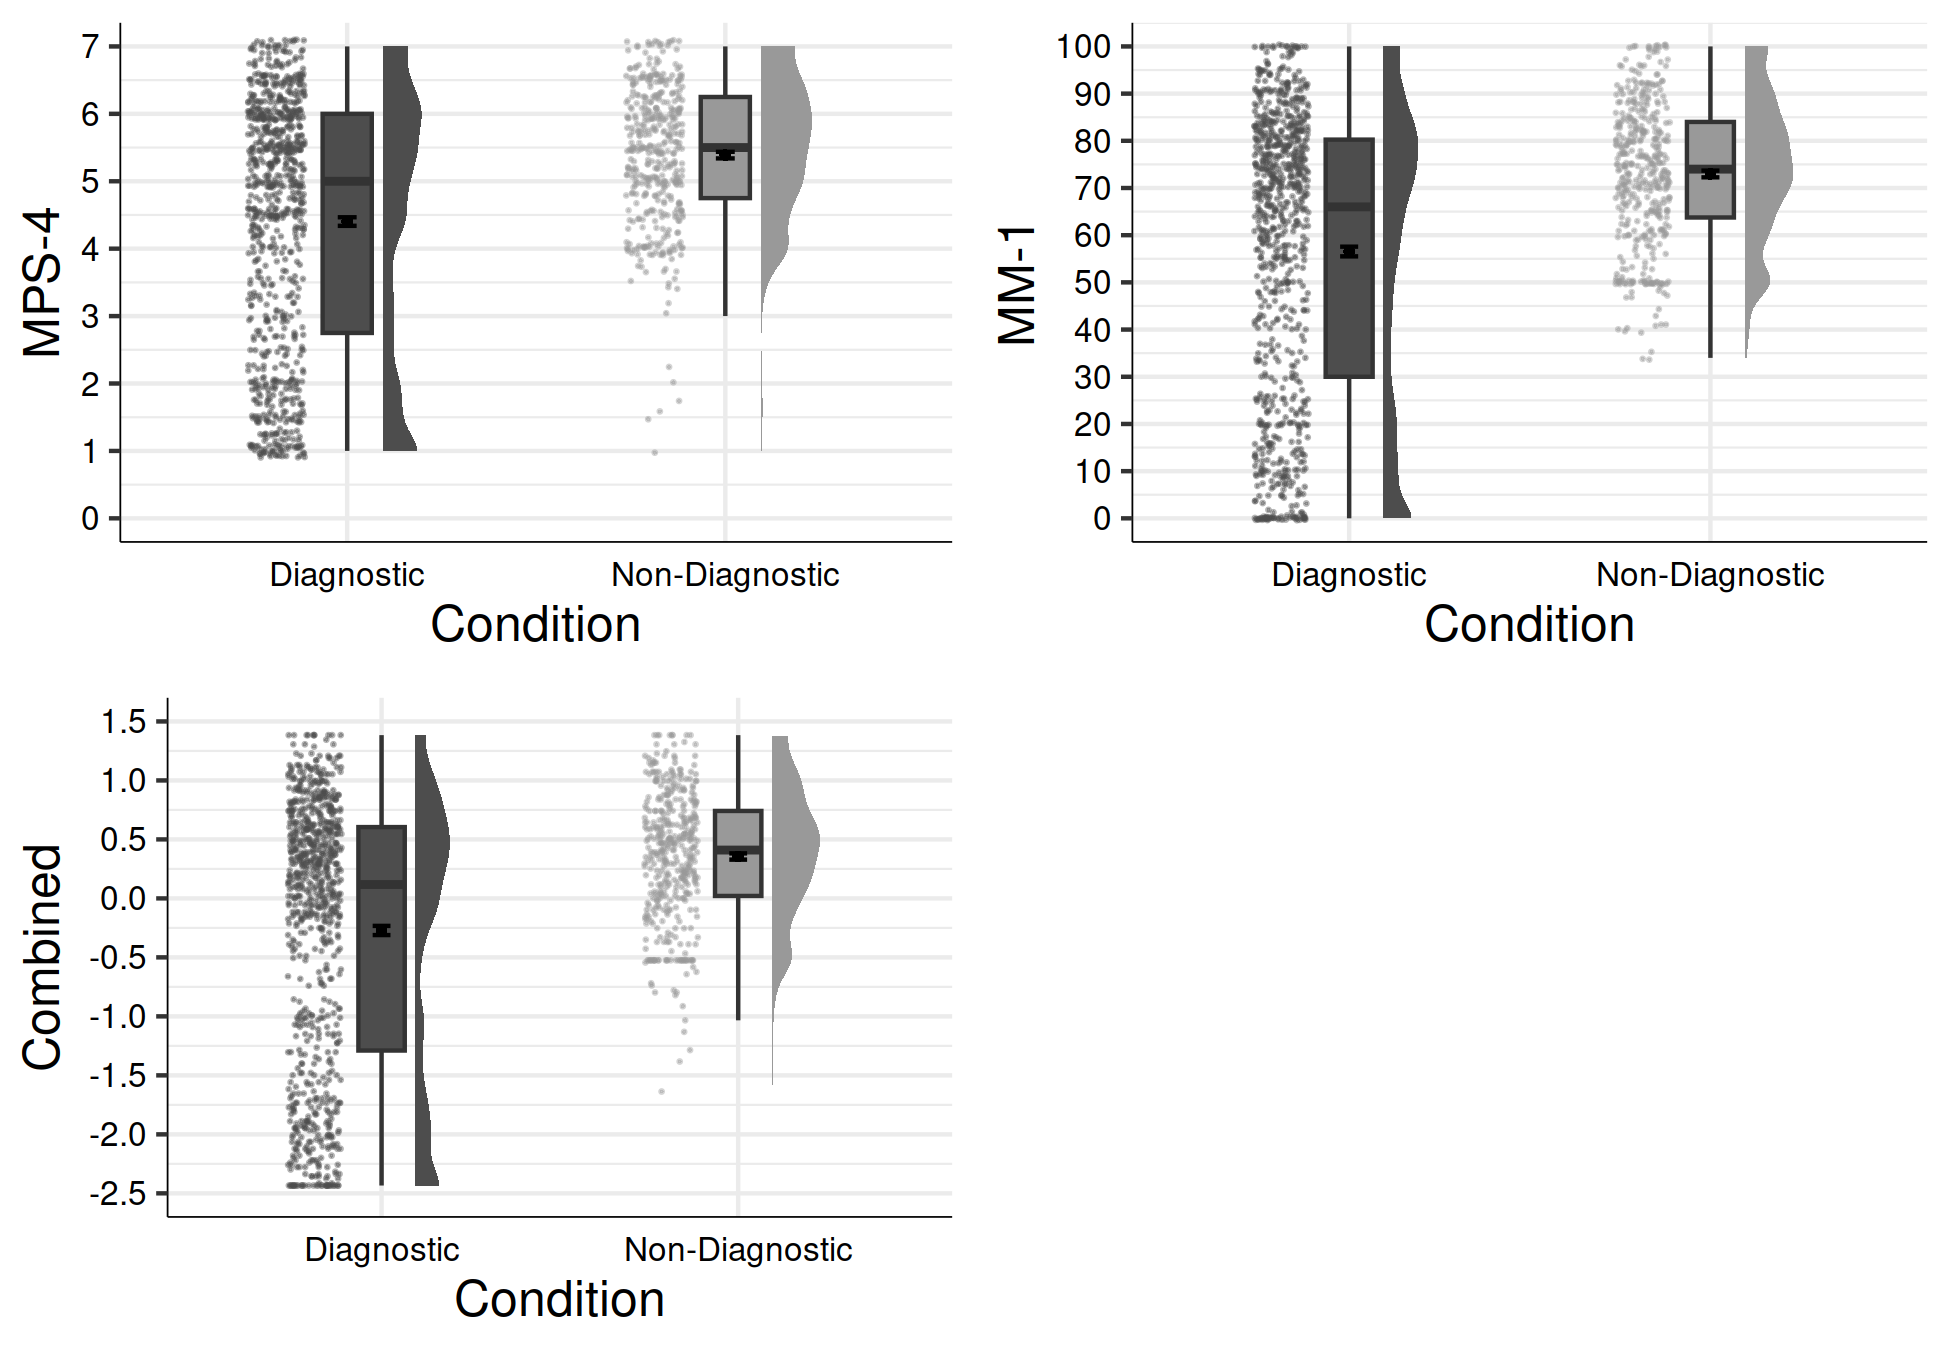
\includegraphics[width=\textwidth,]{Supplementary_files/figure-latex/pilot1bothconditionplot-1} \caption{Pilot Study 1: Differences in moral perception depending on condition}\label{fig:pilot1bothconditionplot}
\end{figure}

We conducted a linear-mixed-effects model to test if condition influenced MM-1 responses. Our outcome measure was MM-1, our predictor variable was condition; we allowed intercepts and the effect of condition to vary across participants. Overall, the model significantly predicted participants responses, and provided a better fit for the data than the baseline model, \(\chi\)\textsuperscript{2}(2) = 924.82, \emph{p} \textless{} .001. Condition was a significant predictor in the model \(b\) = -8.22, \emph{t}(210.98) = -8.60, \emph{p} \textless{} .001, with the non-diagnostic descriptions being rated as more moral than the diagnostic descriptions, see Figure~\ref{fig:pilot1bothconditionplot}.

\subsubsection{Pilot 1: Combined Measure}\label{pilot-1-combined-measure}

We developed a combined moral perception measure by calculating the mean of the combined mean-centered scores for MPS-4 and MM-1, and mean-centering this result. Below we report the analyses for this combined measure.

The standardized means and standard deviations for the combined measure for each scenario are as follows:
\emph{Sam} (diagnostic),
\emph{M} = -0.30, \emph{SD} = 1.16;
\emph{Francis} (diagnostic),
\emph{M} = -0.22, \emph{SD} = 1.06;
\emph{Alex} (diagnostic),
\emph{M} = -0.25, \emph{SD} = 1.10;
\emph{Robin} (diagnostic),
\emph{M} = -0.31, \emph{SD} = 1.19;
\emph{Jackie} (non-diagnostic),
\emph{M} = 0.36, \emph{SD} = 0.55;
\emph{Charlie} (non-diagnostic),
\emph{M} = 0.35, \emph{SD} = 0.55. For the moral descriptions, we observed significant variation depending on the description, \emph{F}(3,602) = 2.67, \emph{p} = .050, partial \(\eta\)\textsuperscript{2} = 0.001. When correcting for multiple comparisons, pairwise comparisons did not reveal significant differences between descriptions. We note that without correction, \emph{Francis} appeared to be rated as more moral than both \emph{Robin} (\emph{p} = .022), and \emph{Sam} (\emph{p} = .021). For the neutral descriptions there was no significant difference in ratings depending on description, \emph{t}(211) = -0.46, \emph{p} = .645, \emph{d} = 0.03.

We conducted a linear-mixed-effects model to test if condition influenced responses on this combined measure. Overall, the model significantly predicted participants responses, and provided a better fit for the data than the baseline model \(\chi\)\textsuperscript{2}(2) = 1,035.36, \emph{p} \textless{} .001, and condition was a significant predictor in the model \(b\) = -0.31, \emph{t}(210.99) = -8.74, \emph{p} \textless{} .001. Participants rated the neutral/non-diagnostic descriptions as more moral than the immoral/diagnostic descriptions (see Figure~\ref{fig:pilot1bothconditionplot}).

\pagebreak

\section{Pilot Study 2}\label{pilot-study-2}

Pilot Study 1 developed materials for studying the dilution effect with morally \emph{bad} characters. In Pilot Study 2, we develop materials for studying the dilution effect with morally \emph{good} characters. As with Pilot Study 1, we developed diagnostic and non-diagnostic descriptions. We hypothesized that evaluations of the diagnostic descriptions would be more extreme (more moral) than for the non-diagnostic descriptions

\subsection{Pilot Study 2: Method}\label{pilot-study-2-method}

\subsubsection{Pilot 2: Participants and design}\label{pilot-2-participants-and-design}

The pilot study was a within-subjects design. The independent variable was description type with two levels, \emph{diagnostic} and \emph{non-diagnostic}. We used the same two dependent variables as in previous studies, the four item moral perception scale (MPS-4, \(\alpha\) = 0.84), and the single item moral perception measure (MM-1).

A total sample of 245 (70 female, 175 male, 0 non-binary, 0 prefer not to say; \emph{M}\textsubscript{age} = 36.69, min = 18, max = 71, \emph{SD} = 9.57) started the survey. Participants were recruited from MTurk.

We removed participants who failed both manipulation checks (\emph{n} = 30), leaving a total sample of 215 participants (63 female, 152 male, 0 non-binary, 0 prefer not to say; \emph{M}\textsubscript{age} = 36.59, min = 18, max = 71, \emph{SD} = 9.59).

\subsubsection{Pilot 2: Procedure and materials}\label{pilot-2-procedure-and-materials}

Data were collected using an online questionnaire presented with Qualtrics (www.qualtrics.com). Participants were presented with descriptions of six characters.

Moral character descriptions were developed by combining descriptions relating to three different moral foundations, focusing on upholding the moral foundations (rather than transgressions as in previous studies). We developed 4 descriptions of moral characters that read as follows:

\begin{enumerate}
\def\labelenumi{(\roman{enumi})}
\tightlist
\item
  \emph{Imagine a person named Sam. Throughout their life they have been known to always help and care for others, treat everyone fairly and equally, and show a strong sense of loyalty to others};
\item
  \emph{Imagine a person named Robin. Throughout their life they have been known to show compassion and empathy for others, act with a sense of fairness and justice, and, never to break their word};
\item
  \emph{Imagine a person named Francis. Throughout their life they have been known to uphold the standards of purity and decency, show respect for authority, and to always act honestly and fairly};
\item
  \emph{Imagine a person named Alex. Throughout their life they have been known to protect and provide shelter to the weak and vulnerable, uphold the rights of others, and show respect for authority}.
\end{enumerate}

We developed 2 descriptions of morally neutral characters that included information relating to physical appearance/attributes, hobbies/activities, and a color preference:

\begin{enumerate}
\def\labelenumi{(\roman{enumi})}
\tightlist
\item
  \emph{Imagine a person named Jackie. They have dark hair, go for a jog twice a week, and their favourite colour is blue};
\item
  \emph{Imagine a person named Charlie. They have blue eyes, drink coffee in the morning, and their favourite colour is green}.
\end{enumerate}

We used the same gender ambiguous names, and we did not specify the gender of the characters. Pilot Study 2 was pre-registered at \color{blue}\url{https://aspredicted.org/W52_VPX}\color{black}.

\subsection{Pilot 2: Results}\label{pilot-2-results}

\subsubsection{Pilot 2: Main Measures}\label{pilot-2-main-measures}

The means and standard deviations for MPS-4 for each scenario are as follows:
\emph{Sam} (diagnostic),
\emph{M}\textsubscript{MPS-4} = 6.01, \emph{SD}\textsubscript{MPS-4} = 0.91,
\emph{Francis} (diagnostic),
\emph{M}\textsubscript{MPS-4} = 5.89, \emph{SD}\textsubscript{MPS-4} = 0.95,
\emph{Alex} (diagnostic),
\emph{M}\textsubscript{MPS-4} = 5.94, \emph{SD}\textsubscript{MPS-4} = 0.94,
\emph{Robin} (diagnostic),
\emph{M}\textsubscript{MPS-4} = 5.93, \emph{SD}\textsubscript{MPS-4} = 0.92,
\emph{Jackie} (non-diagnostic),
\emph{M}\textsubscript{MPS-4} = 5.60, \emph{SD}\textsubscript{MPS-4} = 0.99,
\emph{Charlie} (non-diagnostic),
\emph{M}\textsubscript{MPS-4} = 5.53, \emph{SD}\textsubscript{MPS-4} = 1.08. For the diagnostic descriptions, there was significant variation depending on the description, \emph{F}(3,613) = 2.91, \emph{p} = .036, partial \(\eta\)\textsuperscript{2} = 0.00, \emph{Sam} was viewed significantly more favorably than \emph{Francis} (\emph{p} = .040). For the non-diagnostic descriptions there was no significant difference in ratings depending on description, \emph{t}(214) = -1.79, \emph{p} = .075, \emph{d} = 0.12.

The means and standard deviations for MM-1 for each scenario are as follows:
\emph{Sam} (diagnostic),
\emph{M}\textsubscript{MM-1} = 79.85, \emph{SD}\textsubscript{MM-1} = 15.44;
\emph{Francis} (diagnostic),
\emph{M}\textsubscript{MM-1} = 78.30, \emph{SD}\textsubscript{MM-1} = 15.84;
\emph{Alex} (diagnostic),
\emph{M}\textsubscript{MM-1} = 79.78, \emph{SD}\textsubscript{MM-1} = 15.71;
\emph{Robin} (diagnostic),
\emph{M}\textsubscript{MM-1} = 79.46, \emph{SD}\textsubscript{MM-1} = 15.41;
\emph{Jackie} (non-diagnostic),
\emph{M}\textsubscript{MM-1} = 73.44, \emph{SD}\textsubscript{MM-1} = 15.83;
\emph{Charlie} (non-diagnostic),
\emph{M}\textsubscript{MM-1} = 73.07, \emph{SD}\textsubscript{MM-1} = 16.22. For the diagnostic descriptions, we observed no significant variation depending on the description, \emph{F}(3,594) = 1.45, \emph{p} = .231, partial \(\eta\)\textsuperscript{2} = 0.002. For the non-diagnostic descriptions there was no significant difference in ratings depending on description, \emph{t}(214) = -0.60, \emph{p} = .552, \emph{d} = 0.04.

\begin{figure}[!h]
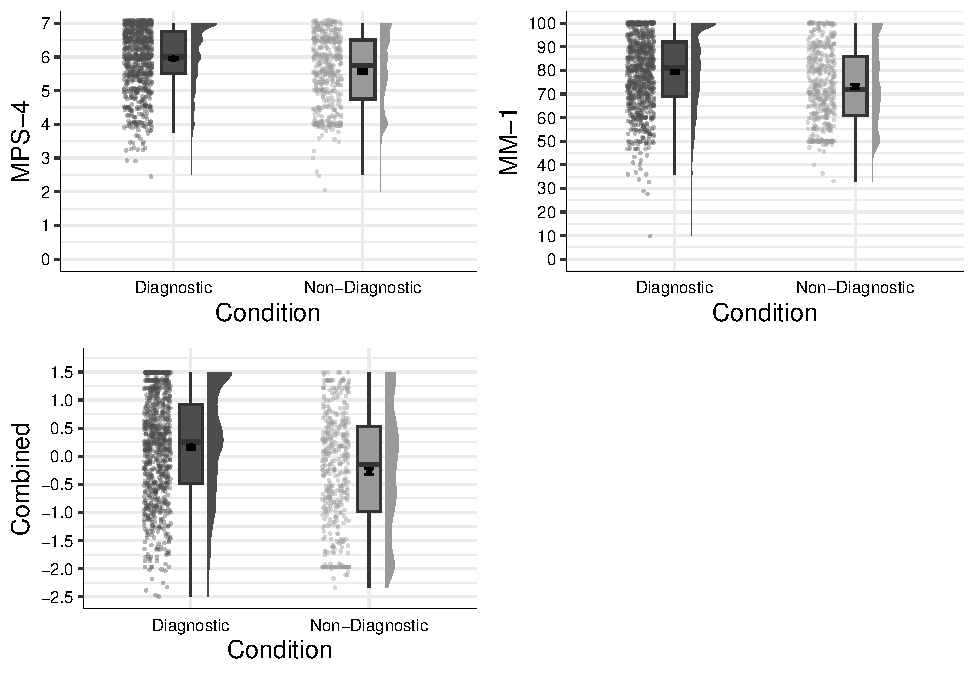
\includegraphics[width=\textwidth,]{Supplementary_files/figure-latex/pilot2bothconditionplot-1} \caption{Pilot Study 2: Differences in moral perception depending on condition}\label{fig:pilot2bothconditionplot}
\end{figure}

We conducted a linear-mixed-effects model to test if condition influenced MPS-4 responses. Our outcome measure was MPS-4, our predictor variable was condition; we allowed intercepts and the effect of condition to vary across participants.
Overall, the model significantly predicted participants responses, and provided a better fit for the data than the baseline model, \(\chi\)\textsuperscript{2}(2) = 475.42, \emph{p} \textless{} .001. Condition was a significant predictor in the model \(b\) = 0.19, \emph{t}(214.35) = 6.53, \emph{p} \textless{} .001, with the diagnostic descriptions being rated as more moral than the non-diagnostic descriptions of immoral characters Figure~\ref{fig:pilot2bothconditionplot}.

We conducted a linear-mixed-effects model to test if condition influenced MM-1 responses. Our outcome measure was MM-1, our predictor variable was condition; we allowed intercepts and the effect of condition to vary across participants. Overall, the model significantly predicted participants responses, and provided a better fit for the data than the baseline model, \(\chi\)\textsuperscript{2}(2) = 324.13, \emph{p} \textless{} .001. Condition was a significant predictor in the model \(b\) = 3.04, \emph{t}(214.90) = 6.02, \emph{p} \textless{} .001, with the diagnostic descriptions being rated as more moral than the non-diagnostic descriptions, see Figure~\ref{fig:pilot2bothconditionplot}.

\subsubsection{Pilot 2: Combined Measure}\label{pilot-2-combined-measure}

As in previous studies, we developed a combined moral perception measure by calculating the mean of the combined mean-centered scores for MPS-4 and MM-1, and mean-centering this result. Below we report the analyses for this combined measure.

The standardized means and standard deviations for the combined measure for each scenario are as follows:
\emph{Sam} (moral),
\emph{M} = 0.21, \emph{SD} = 0.91;
\emph{Francis} (moral),
\emph{M} = 0.10, \emph{SD} = 0.96;
\emph{Alex} (moral),
\emph{M} = 0.18, \emph{SD} = 0.94;
\emph{Robin} (moral),
\emph{M} = 0.16, \emph{SD} = 0.93;
\emph{Jackie} (neutral),
\emph{M} = -0.24, \emph{SD} = 1.01;
\emph{Charlie} (neutral),
\emph{M} = -0.30, \emph{SD} = 1.07. For the moral descriptions, we observed significant variation depending on the description, \emph{F}(3,588) = 2.90, \emph{p} = .039, partial \(\eta\)\textsuperscript{2} = 0.002. \emph{Sam} was viewed significantly more favorably than \emph{Francis} (\emph{p} = .045). For the neutral descriptions there was no significant difference in ratings depending on description, \emph{t}(426.74) = -0.51, \emph{p} = .609, \emph{d} = 0.10.

We conducted a linear-mixed-effects model to test if condition influenced responses to the combined measure. Overall, the model significantly predicted participants responses, and provided a better fit for the data than the baseline model \(\chi\)\textsuperscript{2}(2) = 564.98, \emph{p} \textless{} .001, and condition was a significant predictor in the model \(b\) = 0.22, \emph{t}(214.32) = 6.60, \emph{p} \textless{} .001 (see Figure~\ref{fig:pilot2bothconditionplot}).

\pagebreak

\section{Study S1 - Good Characters}\label{study-s1---good-characters}

Study S1 is a replication of Study 2, but with an MTurk Sample.

\subsection{Study S1: Method}\label{study-s1-method}

\subsubsection{Study S1: Participants and design}\label{study-s1-participants-and-design}

The design, materials, and procedure for Study S1 were the same as for Study 2, the only change from Study 2 was that all participants in Study S2 were recruited from MTurk. Study S1 was a within-subjects design. The independent variable was condition with two levels, diagnostic and non-diagnostic. We used the same two dependent variables as in previous studies, the four item moral perception scale (MPS-4, \(\alpha\) = 0.81), and the single item moral perception measure MM-1.

A total sample of 1118 (445 female, 642 male, 2 non-binary, 3 other; 1 prefer not to say, \emph{M}\textsubscript{age} = 37.44, min = 19, max = 84, \emph{SD} = 11.08) started the survey. Participants were recruited from MTurk and paid \$0.40 for their participation.

Participants who failed both manipulation checks were removed (\emph{n} = 262), leaving a total sample of 856 participants (347 female, 507 male, 0 other, 0 prefer not to say; \emph{M}\textsubscript{age} = 37.12, min = 19, max = 84, \emph{SD} = 11.04).

\subsubsection{Study S1: Procedure and materials}\label{study-s1-procedure-and-materials}

All materials and procedures were the same as in Study 2.

\subsection{Study S1: Results}\label{study-s1-results}

\subsubsection{Study S1: Main Measures}\label{study-s1-main-measures}

The means and standard deviations for MPS-4 for each scenario are as follows:
\emph{Sam},
\emph{M}\textsubscript{MPS-4} = 5.95, \emph{SD}\textsubscript{MPS-4} = 0.93,
\emph{Francis},
\emph{M}\textsubscript{MPS-4} = 5.89, \emph{SD}\textsubscript{MPS-4} = 0.91,
\emph{Alex},
\emph{M}\textsubscript{MPS-4} = 5.94, \emph{SD}\textsubscript{MPS-4} = 0.96,
\emph{Robin},
\emph{M}\textsubscript{MPS-4} = 5.95, \emph{SD}\textsubscript{MPS-4} = 0.94. There was significant variation depending on the description, \emph{F}(3,2527) = 3.30, \emph{p} = .020, partial \(\eta\)\textsuperscript{2} = 0.001. Pairwise comparisons did not reveal any significant differences between individual descriptions (all \emph{p}s \textgreater{} .05).

The means and standard deviations for MM-1 for each scenario are as follows:
\emph{Sam} (diagnostic/moral),
\emph{M}\textsubscript{MM-1} = 81.34, \emph{SD}\textsubscript{MM-1} = 14.14;
\emph{Francis} (diagnostic/moral),
\emph{M}\textsubscript{MM-1} = 80.65, \emph{SD}\textsubscript{MM-1} = 14.16;
\emph{Alex} (diagnostic/moral),
\emph{M}\textsubscript{MM-1} = 81.15, \emph{SD}\textsubscript{MM-1} = 14.42;
\emph{Robin} (diagnostic/moral),
\emph{M}\textsubscript{MM-1} = 81.63, \emph{SD}\textsubscript{MM-1} = 14.15. There was significant variation depending on the description, \emph{F}(3,2518) = 2.89, \emph{p} = .035, partial \(\eta\)\textsuperscript{2} = 0.001. Pairwise comparisons did not reveal any significant differences between individual descriptions (all \emph{p}s \textgreater{} .05).

We conducted a linear-mixed-effects model to test if condition influenced MPS-4 responses. Our outcome measure was MPS-4, our predictor variable was condition; we allowed intercepts and the effect of condition to vary across participants, and scenario was also included in the model.
Overall, the model significantly predicted participants responses, and provided a better fit for the data than the baseline model, \(\chi\)\textsuperscript{2}(8) = 17.86, \emph{p} = .022. Condition did not influence responses to the MPS-4, \emph{F}(1, 866.60) = 2.80, \emph{p} = .095; and was not a significant predictor in the model when controlling for scenario, \(b\) = 0.01, \emph{t}(867) = 1.67, \emph{p} = .095, see Figure~\ref{fig:S4bothconditionplot}.

\begin{figure}[!h]
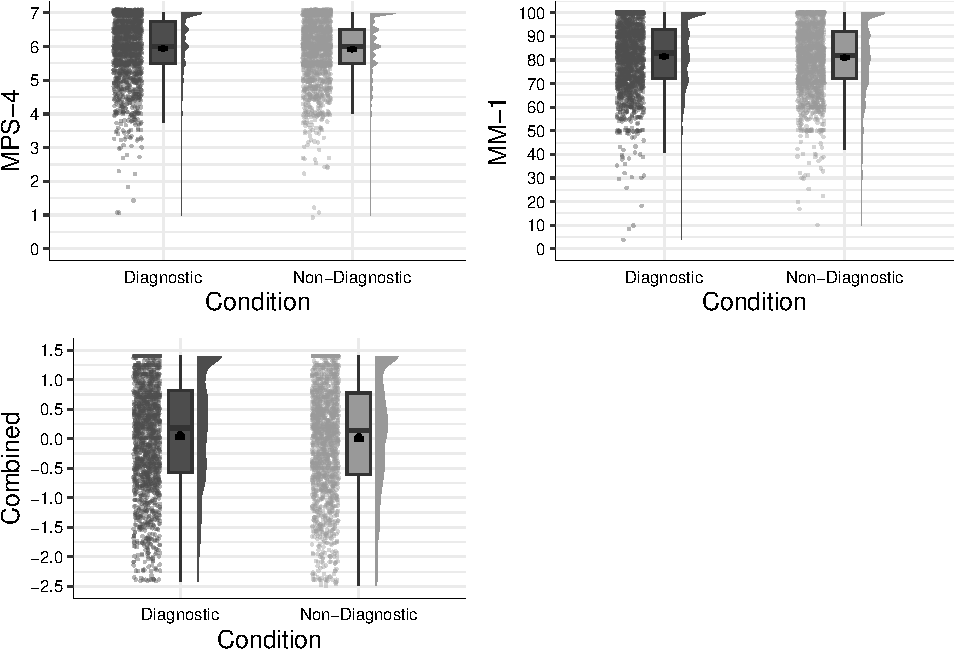
\includegraphics[width=\textwidth,]{Supplementary_files/figure-latex/S4bothconditionplot-1} \caption{Study S1: Responses to moral perception measures depending on condition}\label{fig:S4bothconditionplot}
\end{figure}

We conducted a linear-mixed-effects model to test if condition influenced MM-1 responses. Our outcome measure was MM-1, our predictor variable was condition; we allowed intercepts and the effect of condition to vary across participants. Overall, the model significantly predicted participants responses, and provided a better fit for the data than the baseline model, \(\chi\)\textsuperscript{2}(8) = 40.10, \emph{p} \textless{} .001. Condition significantly influenced MM-1 responses \emph{F}(1, 864) = 4.79, \emph{p} = .029, and was a significant predictor in the model \(b\) = 0.29, \emph{t}(864) = 2.19, \emph{p} = .029, see Figure~\ref{fig:S4bothconditionplot}.

\subsubsection{Study S1: Combined Measure}\label{study-s1-combined-measure}

The means and standard deviations for the combined measure for each scenario are as follows:
\emph{Sam},
\emph{M} = 0.03, \emph{SD} = 1.02,
\emph{Francis},
\emph{M} = -0.03, \emph{SD} = 0.98,
\emph{Alex},
\emph{M} = 0.02, \emph{SD} = 1.04,
\emph{Robin},
\emph{M} = 0.04, \emph{SD} = 1.01. There was significant variation depending on the description, \emph{F}(3,2493) = 4.32, \emph{p} = .005, partial \(\eta\)\textsuperscript{2} = 0.00. Follow-up pairwise comparisons did not reveal any significant differences between the different characters (all \emph{p}s \textgreater{} .05).

We conducted a linear-mixed-effects model to test if condition influenced moral perception. Our outcome measure was the combined moral perception measure, our predictor variable was condition; we allowed intercepts and the effect of condition to vary across participants, and scenario was also included in the model.
Overall, the model significantly predicted participants responses, and provided a better fit for the data than the baseline model, \(\chi\)\textsuperscript{2}(8) = 42.42, \emph{p} \textless{} .001. Condition did not influence moral perception, \emph{F}(1, 865.01) = 5.31, \emph{p} = .021; and was not a significant predictor in the model when controlling for scenario, \(b\) = -0.01, \emph{t}(2,541.03) = -0.82, \emph{p} = .410, see Figure~\ref{fig:S3combinedconditionplot}.

\subsubsection{Study S1: Differences between the Descriptions}\label{study-s1-differences-between-the-descriptions}

Below we provide analyses of the effect of condition on responses to each scenario individually. The responses for each scenario across each measure depending on condition are displayed in Figure~\ref{fig:Supp1AllscenariosPlot}.

\begin{figure}[!h]
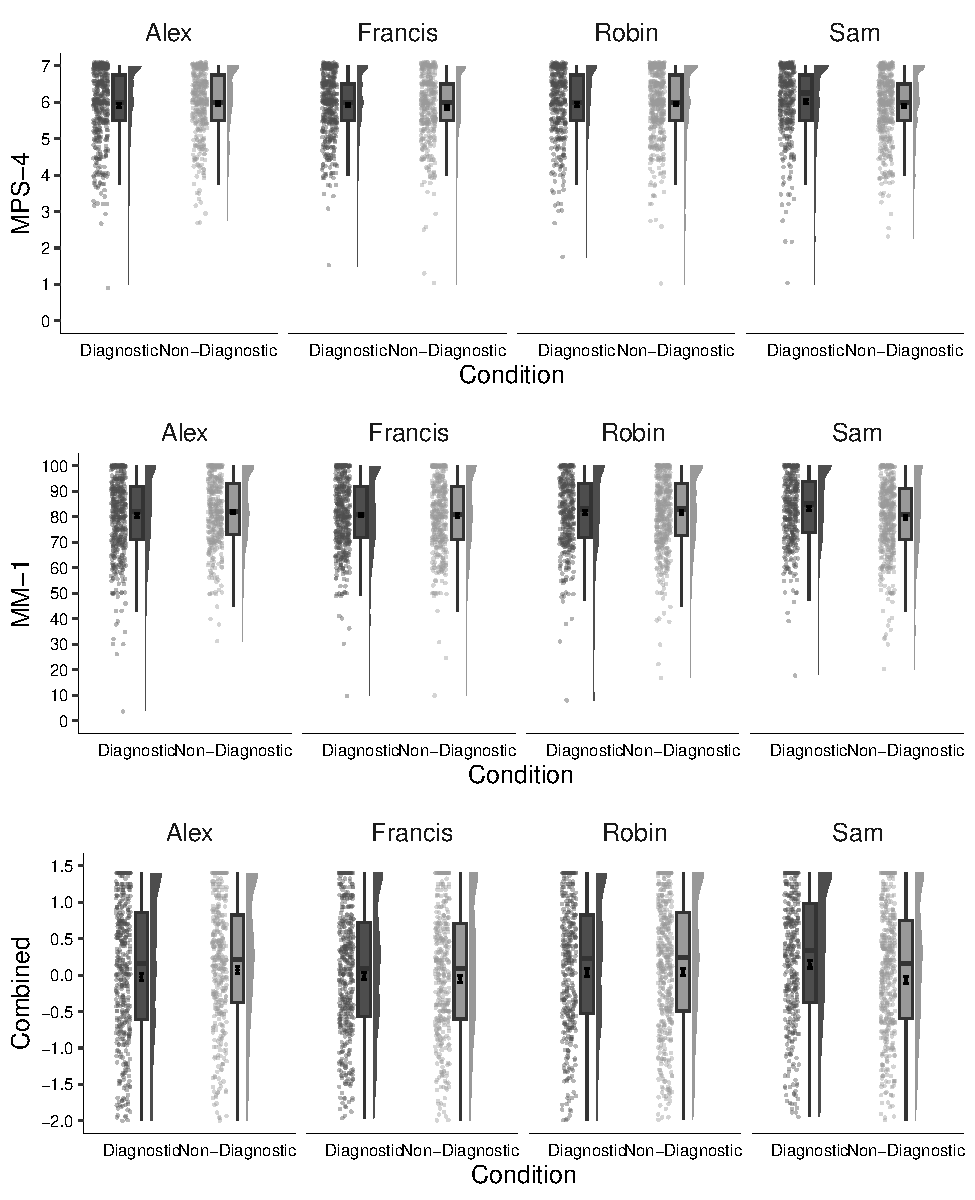
\includegraphics[width=\textwidth,]{Supplementary_files/figure-latex/Supp1AllscenariosPlot-1} \caption{Study 2: Differences in moral perception for each description}\label{fig:Supp1AllscenariosPlot}
\end{figure}

For \emph{Sam}, MPS-4 scores were not significantly different in the non-diagnostic condition (\emph{M} = 5.89, \emph{SD} = 0.91), than in the diagnostic condition (\emph{M} = 6.02, \emph{SD} = 0.95), \emph{t}(810.53) = 1.97, \emph{p} = .049, \emph{d} = 0.14; MM-1 ratings were similar in the non-diagnostic condition (\emph{M} = 79.75, \emph{SD} = 14.62), than in the diagnostic condition (\emph{M} = 83.25, \emph{SD} = 13.30), \emph{t}(845.88) = 3.66, \emph{p} \textless{} .001, \emph{d} = 0.25. For the combined measure ratings were also similar in the non-diagnostic condition (\emph{M} = -0.06, \emph{SD} = 1.03), than in the diagnostic condition (\emph{M} = 0.15, \emph{SD} = 1.01), \emph{t}(829.20) = 3.07, \emph{p} = .002, \emph{d} = 0.21.

For \emph{Robin}, MPS-4 scores were not significantly different for the non-diagnostic condition (\emph{M} = 5.95, \emph{SD} = 0.93), than in the diagnostic condition (\emph{M} = 5.94, \emph{SD} = 0.95), \emph{t}(811.83) = -0.20, \emph{p} = .841, \emph{d} = 0.01; MM-1 ratings were similar in the non-diagnostic condition (\emph{M} = 81.62, \emph{SD} = 14.28), and in the diagnostic condition (\emph{M} = 81.64, \emph{SD} = 14.02), \emph{t}(824.54) = 0.02, \emph{p} = .982, \emph{d} = 0.00. For the combined measure ratings were also similar in the non-diagnostic condition (\emph{M} = 0.04, \emph{SD} = 1.03), than in the diagnostic condition (\emph{M} = 0.04, \emph{SD} = 0.99), \emph{t}(828.47) = -0.10, \emph{p} = .919, \emph{d} = 0.01.

For \emph{Alex}, MPS-4 scores were not significantly different for the non-diagnostic condition (\emph{M} = 5.97, \emph{SD} = 0.91), than in the diagnostic condition (\emph{M} = 5.91, \emph{SD} = 0.99), \emph{t}(845.29) = -0.91, \emph{p} = .362, \emph{d} = 0.06; MM-1 ratings were similar in the non-diagnostic condition (\emph{M} = 81.93, \emph{SD} = 13.38), than in the diagnostic condition (\emph{M} = 80.51, \emph{SD} = 15.21), \emph{t}(850.53) = -1.46, \emph{p} = .145, \emph{d} = 0.10. For the combined measure ratings were also similar in the non-diagnostic condition (\emph{M} = 0.07, \emph{SD} = 0.98), than in the diagnostic condition (\emph{M} = -0.02, \emph{SD} = 1.09), \emph{t}(847.27) = -1.30, \emph{p} = .192, \emph{d} = 0.09.

For \emph{Francis}, MPS-4 scores were not significantly different for the non-diagnostic condition (\emph{M} = 5.87, \emph{SD} = 0.95), than in the diagnostic condition (\emph{M} = 5.91, \emph{SD} = 0.87), \emph{t}(787.36) = 0.77, \emph{p} = .443, \emph{d} = 0.05; MM-1 ratings were not significantly different in the non-diagnostic condition (\emph{M} = 80.54, \emph{SD} = 14.38), than in the diagnostic condition (\emph{M} = 80.75, \emph{SD} = 13.99), \emph{t}(809.63) = 0.21, \emph{p} = .832, \emph{d} = 0.01. For the combined measure ratings were also similar in the non-diagnostic condition (\emph{M} = -0.05, \emph{SD} = 0.99), and in the diagnostic condition (\emph{M} = -0.01, \emph{SD} = 0.98), \emph{t}(814.30) = 0.55, \emph{p} = .581, \emph{d} = 0.04.

\newpage

\newpage

\pagebreak

\section{Study S2 - Good and Bad Characters}\label{study-s2---good-and-bad-characters}

Study S2 is the same as Study 3, but with an MTurk sample. Study 3 was pre-registered at \color{blue}\url{https://aspredicted.org/QDF_XT1}\color{black}.

\subsection{Study S2: Method}\label{study-s2-method}

\subsubsection{Study S2: Participants and design}\label{study-s2-participants-and-design}

Study S2 was a 2 \(\times\) 2 within-subjects factorial design. The first independent variable was condition with two levels, diagnostic and non-diagnostic. The second independent variable was valence of character description, with two levels morally good and morally bad. We used the same two dependent variables as in previous studies, the four item moral perception scale (MPS-4, \(\alpha\) = 0.94), and the single item moral perception measure MM-1.

A total sample of 1095 (386 female, 700 male, 2 non-binary, 0 other; 2 prefer not to say, \emph{M}\textsubscript{age} = 36.42, min = 19, max = 77, \emph{SD} = 10.65) started the survey. Participants were recruited from MTurk and paid \$0.40 for their participation.

Participants who failed both manipulation checks were removed (\emph{n} = 221), leaving a total sample of 874 participants (320 female, 550 male, 0 other, 0 prefer not to say; \emph{M}\textsubscript{age} = 36.37, min = 19, max = 77, \emph{SD} = 10.72).

\subsubsection{Study S2: Procedure and materials}\label{study-s2-procedure-and-materials}

Again, data were collected using an online questionnaire presented with Qualtrics (www.qualtrics.com). Participants were presented with four descriptions of characters as in Study 3. To ensure consistency across character judgments, we selected descriptions that related to the same moral foundations (care, fairness, and loyalty). We used the same four character names as in previous studies. The \emph{good} characters were \emph{Sam} and \emph{Robin}, and the \emph{bad} characters were \emph{Francis} and \emph{Alex}, e.g., \emph{Imagine a person named Robin. Throughout their life they have been known to show compassion and empathy for others, act with a sense of fairness and justice, and, never to break their word.} or, \emph{Imagine a person named Alex. Throughout their life they have been known to be cruel, act unfairly, and to betray their own group.} Full descriptions for each character are in the supplementary materials. One description for each the \emph{good} and \emph{bad} characters was randomly assigned to include non-diagnostic information for each participant thus all participants were exposed to all conditions (see \color{blue}\url{https://osf.io/mdnpv/?view_only=77883e3fbc3d45f1a35fe92d5318cb67}\color{black} for details of the randomization blocks). Study S2 was pre-registered at \color{blue}\url{https://aspredicted.org/QDF_XT1}\color{black}

\subsection{Study S2: Results}\label{study-s2-results}

The means and standard deviations for MPS-4 for each scenario are as follows:
\emph{Sam} (good),
\emph{M}\textsubscript{MPS-4} = 5.90, \emph{SD}\textsubscript{MPS-4} = 1.03,
\emph{Francis} (bad),
\emph{M}\textsubscript{MPS-4} = 4.07, \emph{SD}\textsubscript{MPS-4} = 2.07,
\emph{Alex} (bad),
\emph{M}\textsubscript{MPS-4} = 4.03, \emph{SD}\textsubscript{MPS-4} = 2.03,
\emph{Robin} (good),
\emph{M}\textsubscript{MPS-4} = 5.85, \emph{SD}\textsubscript{MPS-4} = 1.05. There was significant variation depending on the description, \emph{F}(1,1080) = 442.71, \emph{p} \textless{} .001, partial \(\eta\)\textsuperscript{2} = 0.24. Both the \emph{good} characters (\emph{Robin} and \emph{Sam}) were rated significantly more favorably than both the \emph{bad} characters (\emph{Alex} and \emph{Francis}; all \emph{p}s \textless{} .001). There were no differences between \emph{Robin} and \emph{Sam} (\emph{good}: \emph{p} = .366) or between \emph{Alex} and \emph{Francis} (\emph{bad}; \emph{p} = .648).

The means and standard deviations for MM-1 for each scenario are as follows:
\emph{Sam} (good),
\emph{M}\textsubscript{MM-1} = 81.01, \emph{SD}\textsubscript{MM-1} = 15.23;
\emph{Francis} (bad),
\emph{M}\textsubscript{MM-1} = 51.49, \emph{SD}\textsubscript{MM-1} = 33.18;
\emph{Alex} (bad),
\emph{M}\textsubscript{MM-1} = 50.89, \emph{SD}\textsubscript{MM-1} = 32.14;
\emph{Robin} (good),
\emph{M}\textsubscript{MM-1} = 80.81, \emph{SD}\textsubscript{MM-1} = 15.16. There was significant variation depending on the description, \emph{F}(1,1080) = 458.92, \emph{p} \textless{} .001, partial \(\eta\)\textsuperscript{2} = 0.254. Again, the \emph{good} characters (\emph{Robin} and \emph{Sam}) were rated significantly more favorably than the \emph{bad} characters (\emph{Alex} and \emph{Francis}; all \emph{p}s \textless{} .001). There were no differences between \emph{Robin} and \emph{Sam} (\emph{good}: \emph{p} = .776) or between \emph{Alex} and \emph{Francis} (\emph{bad}; \emph{p} = .683).

We conducted a linear-mixed-effects model to test if our predictors influenced MPS-4 responses. Our outcome measure was MPS-4, our predictor variables were condition and valence; we allowed intercepts and the effects of condition and valence to vary across participants.
Overall, the model significantly predicted participants responses, and provided a better fit for the data than the baseline model,
\(\chi\)\textsuperscript{2}(5) = 4,554.31, \emph{p} \textless{} .001.
Overall, there was a significant main effect for condition,
\emph{F}(1, 873) = 8.61, \emph{p} = .003;
valence significantly predicted responses,
\emph{F}(1, 873) = 1,859.34, \emph{p} \textless{} .001;
and there was no significant condition \(\times\) valence interaction,
\emph{F}(1, 873) = 0.01, \emph{p} = .935.

We conducted a linear-mixed-effects model to test if our predictors influenced MM-1 responses. The model was the same as the previous model, with a change to the outcome measure, our outcome measure for this model was MM-1. As above, our predictor variables were condition and valence; we allowed intercepts and the effects of condition and valence to vary across participants.
Overall, the model significantly predicted participants responses, and provided a better fit for the data than the baseline model,
\(\chi\)\textsuperscript{2}(5) = 3,496.86, \emph{p} \textless{} .001.
Overall there was a main effect for condition,
\emph{F}(1, 873) = 16.61, \emph{p} \textless{} .001;
valence significantly predicted responses,
\emph{F}(1, 873) = 986.37, \emph{p} \textless{} .001;
and there was no significant condition \(\times\) valence interaction,
\emph{F}(1, 873) = 0.04, \emph{p} = .849.

We conducted a linear-mixed-effects model to test if our predictors influenced responses on the combined moral perception measure. Our outcome measure was the combined moral perception measure, our predictor variables were condition and valence; we allowed intercepts and the effects of condition and valence to vary across participants.
Overall, the model significantly predicted participants responses, and provided a better fit for the data than the baseline model,
\(\chi\)\textsuperscript{2}(5) = 4,467.15, \emph{p} \textless{} .001.
Condition significantly influenced responses to the combined moral perception measure,
\emph{F}(1, 873) = 16.65, \emph{p} \textless{} .001
and was a significant predictor in the model when controlling for scenario, \(b\) = -0.02, \emph{t}(873.00) = -4.08, \emph{p} \textless{} .001;
valence significantly predicted responses,
\emph{F}(1, 873) = 1,598.27, \emph{p} \textless{} .001;
and there was also a significant condition \(\times\) valence interaction,
\emph{F}(1, 873) = 0.03, \emph{p} = .867, see Figure~\ref{fig:S3combinedplot}.

For both MP-4 and MM-1 (and the combined measure) we found a main effect for condition and valence, and there was no condition \(\times\) valence interaction. We conducted follow-up analyses to test the if the main effect for condition holds for both good and bad descriptions separately.

\begin{figure}[!h]
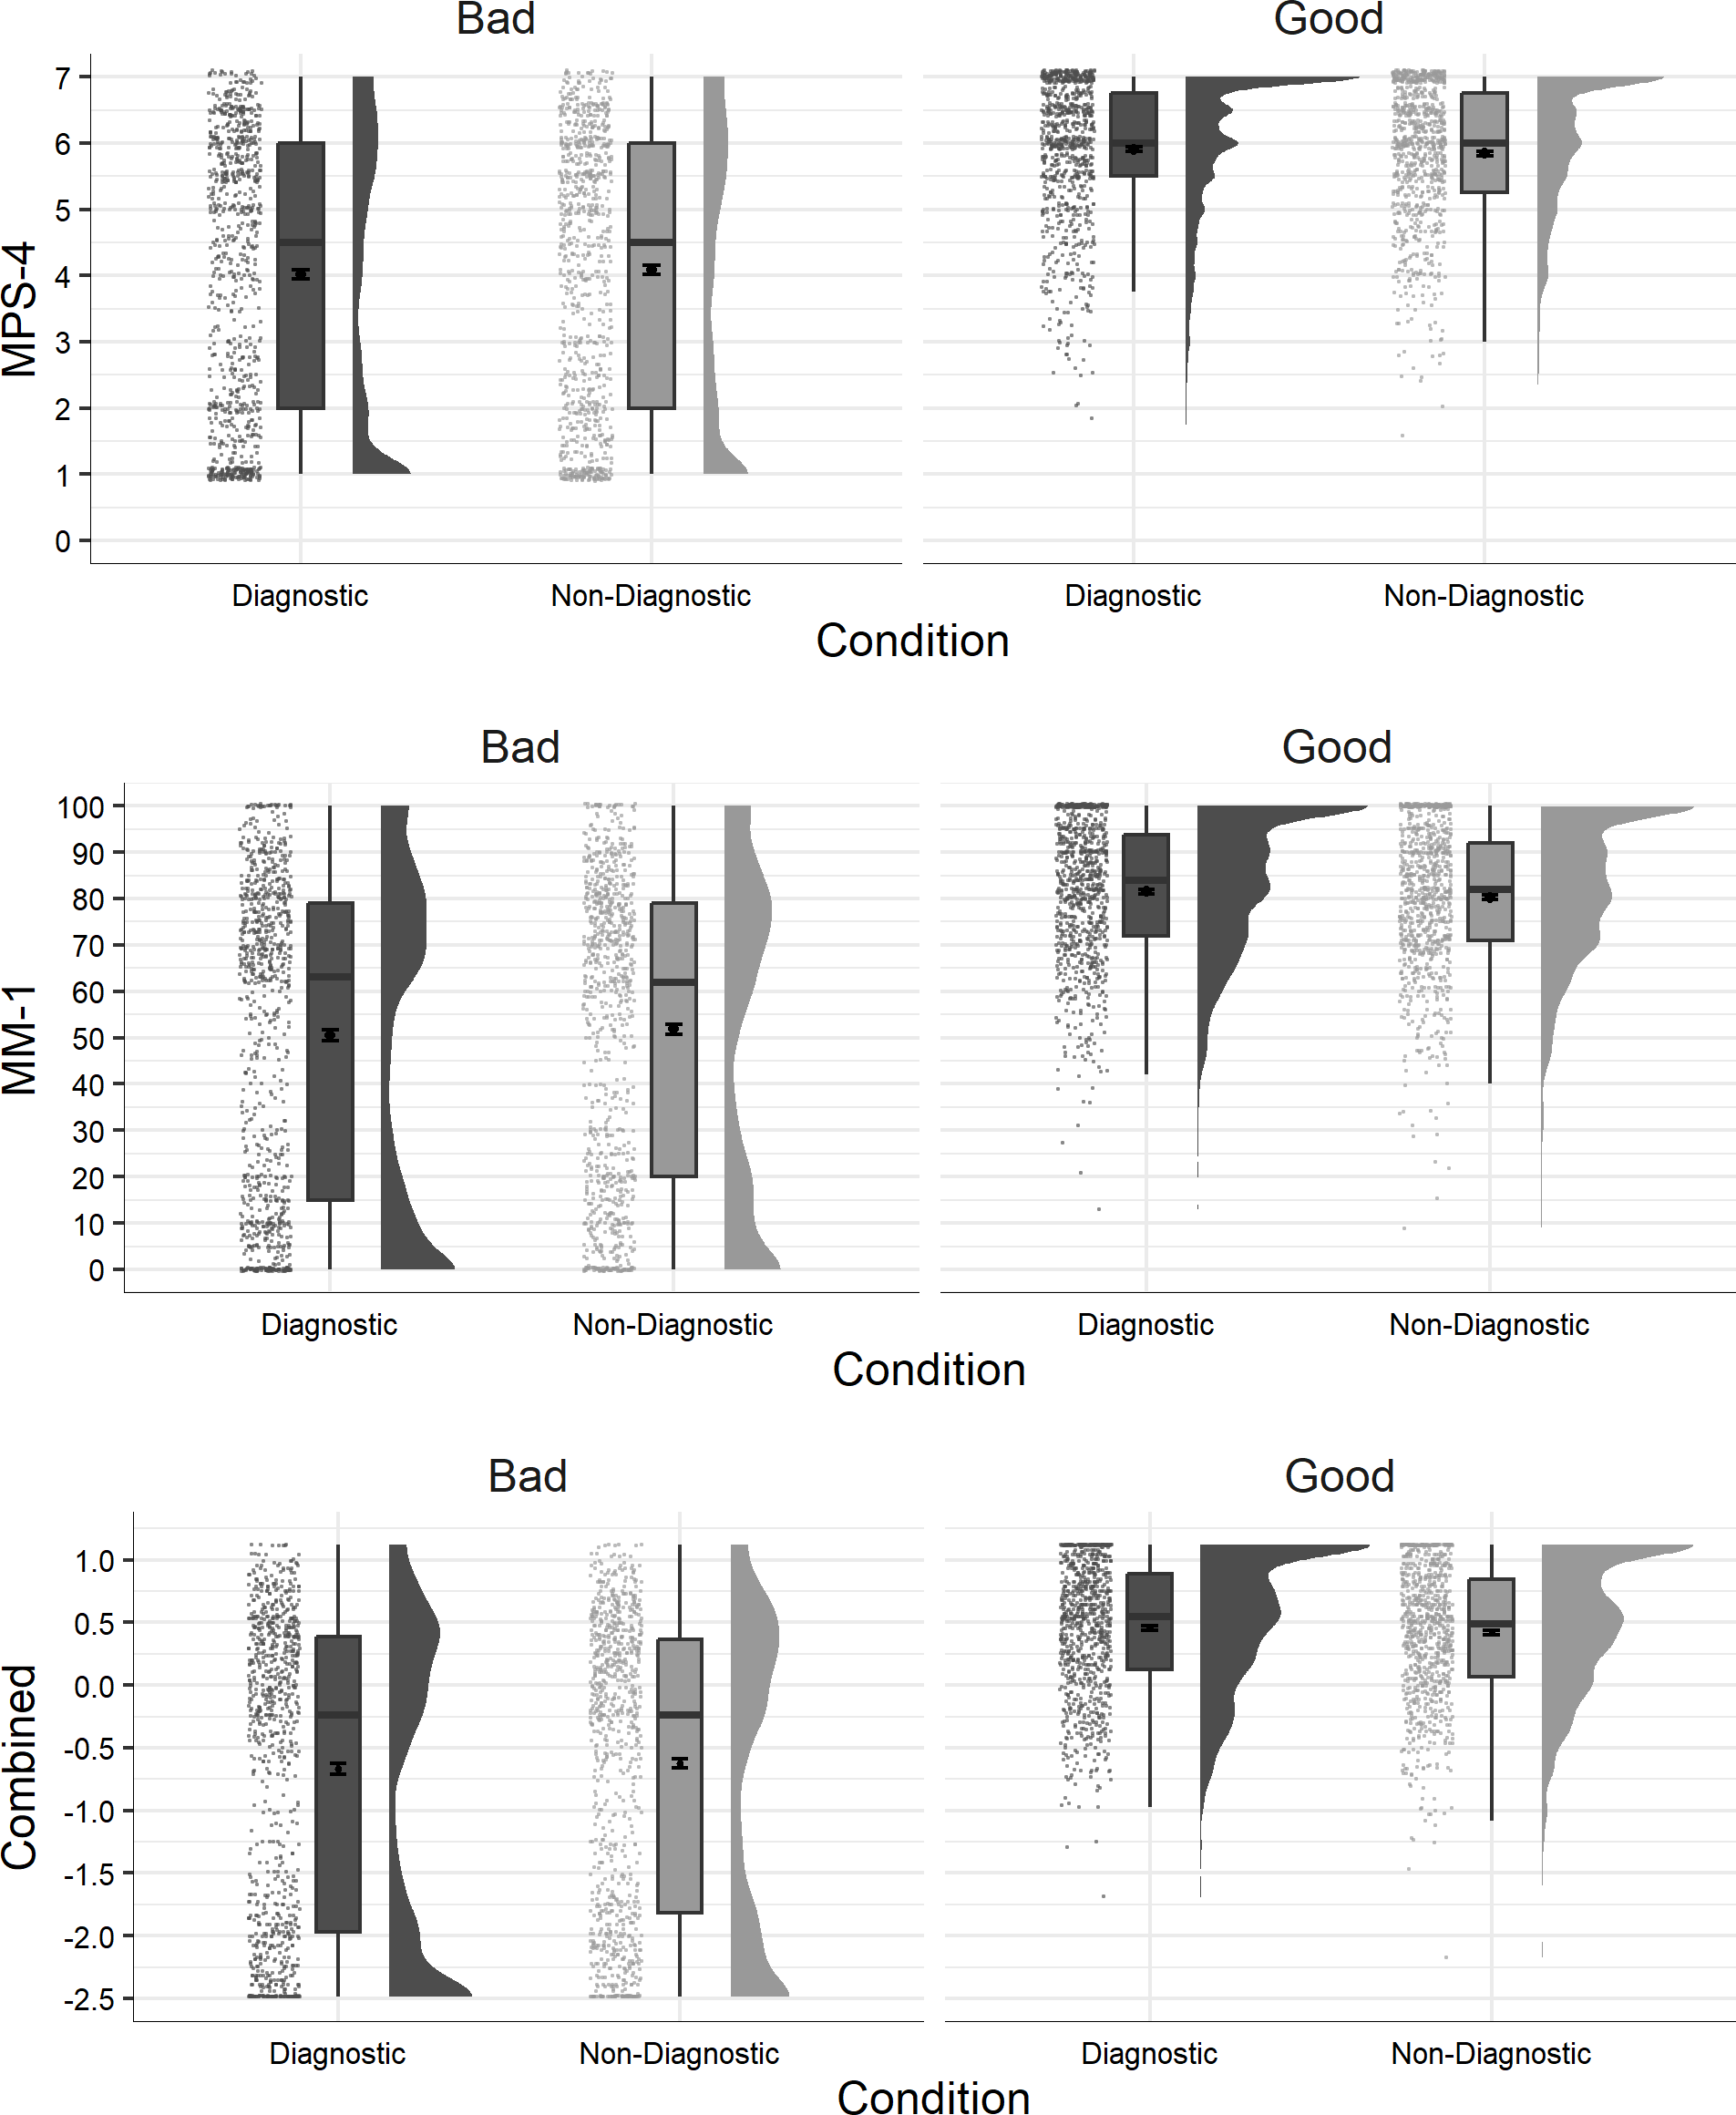
\includegraphics[width=\textwidth,]{Supplementary_files/figure-latex/StudyS2bothconditionplot-1} \caption{Study S2: Differences in moral perception depending on condition}\label{fig:StudyS2bothconditionplot}
\end{figure}

\subsection{\texorpdfstring{Differences in the \emph{Bad} Descriptions}{Differences in the Bad Descriptions}}\label{differences-in-the-bad-descriptions}

For the \emph{bad} characters, we conducted a linear-mixed-effects model to test if condition influenced MPS-4 responses. Our outcome measure was MPS-4, our predictor variable was condition; we allowed intercepts and the effect of condition to vary across participants. Overall, the model did not significantly predict participants responses, or provide a better fit for the data than the baseline model, \(\chi\)\textsuperscript{2}(3) = 5.40, \emph{p} = .145. Condition did not significantly influence MPS-4 responses \emph{F}(1, 872.00) = 3.54, \emph{p} = .060, and was not a significant predictor in the model \(b\) = -0.03, \emph{t}(872.00) = -1.88, \emph{p} = .060, see Figure~\ref{fig:StudyS2bothconditionplot}.

We also conducted a linear-mixed-effects model to test if condition influenced MM-1 responses. Our outcome measure was MM-1, our predictor variable was condition; we allowed intercepts and the effect of condition to vary across participants. Overall, the model significantly predicted participants responses, and provided a better fit for the data than the baseline model, \(\chi\)\textsuperscript{2}(3) = 8.67, \emph{p} = .034. Condition significantly influenced MM-1 responses \emph{F}(1, 872.00) = 7.01, \emph{p} = .008, and was a significant predictor in the model \(b\) = -0.69, \emph{t}(872.00) = -2.65, \emph{p} = .008, see Figure~\ref{fig:StudyS2bothconditionplot}.

\subsection{\texorpdfstring{Differences in the \emph{Good} Descriptions}{Differences in the Good Descriptions}}\label{differences-in-the-good-descriptions}

For the \emph{good} characters, we conducted a linear-mixed-effects model to test if condition influenced MPS-4 responses. Our outcome measure was MPS-4, our predictor variable was condition; we allowed intercepts and the effect of condition to vary across participants. Overall, the model significantly predicted participants responses, and provided a better fit for the data than the baseline model, \(\chi\)\textsuperscript{2}(3) = 13.66, \emph{p} = .003. Condition significantly influenced MPS-4 responses \emph{F}(1, 872.00) = 6.82, \emph{p} = .009, and was a significant predictor in the model \(b\) = 0.03, \emph{t}(872.00) = 2.61, \emph{p} = .009, see Figure~\ref{fig:StudyS2bothconditionplot}.

We conducted a linear-mixed-effects model to test if condition influenced MM-1 responses. Our outcome measure was MM-1, our predictor variable was condition; we allowed intercepts and the effect of condition to vary across participants. Overall, the model significantly predicted participants responses, and provided a better fit for the data than the baseline model, \(\chi\)\textsuperscript{2}(1) = 11.97, \emph{p} \textless{} .001. Condition significantly influenced MM-1 responses \emph{F}(1, 873) = 12.04, \emph{p} \textless{} .001, and was a significant predictor in the model \(b\) = 0.63, \emph{t}(873) = 3.47, \emph{p} \textless{} .001, see Figure~\ref{fig:StudyS2bothconditionplot}.

\begin{figure}[!p]
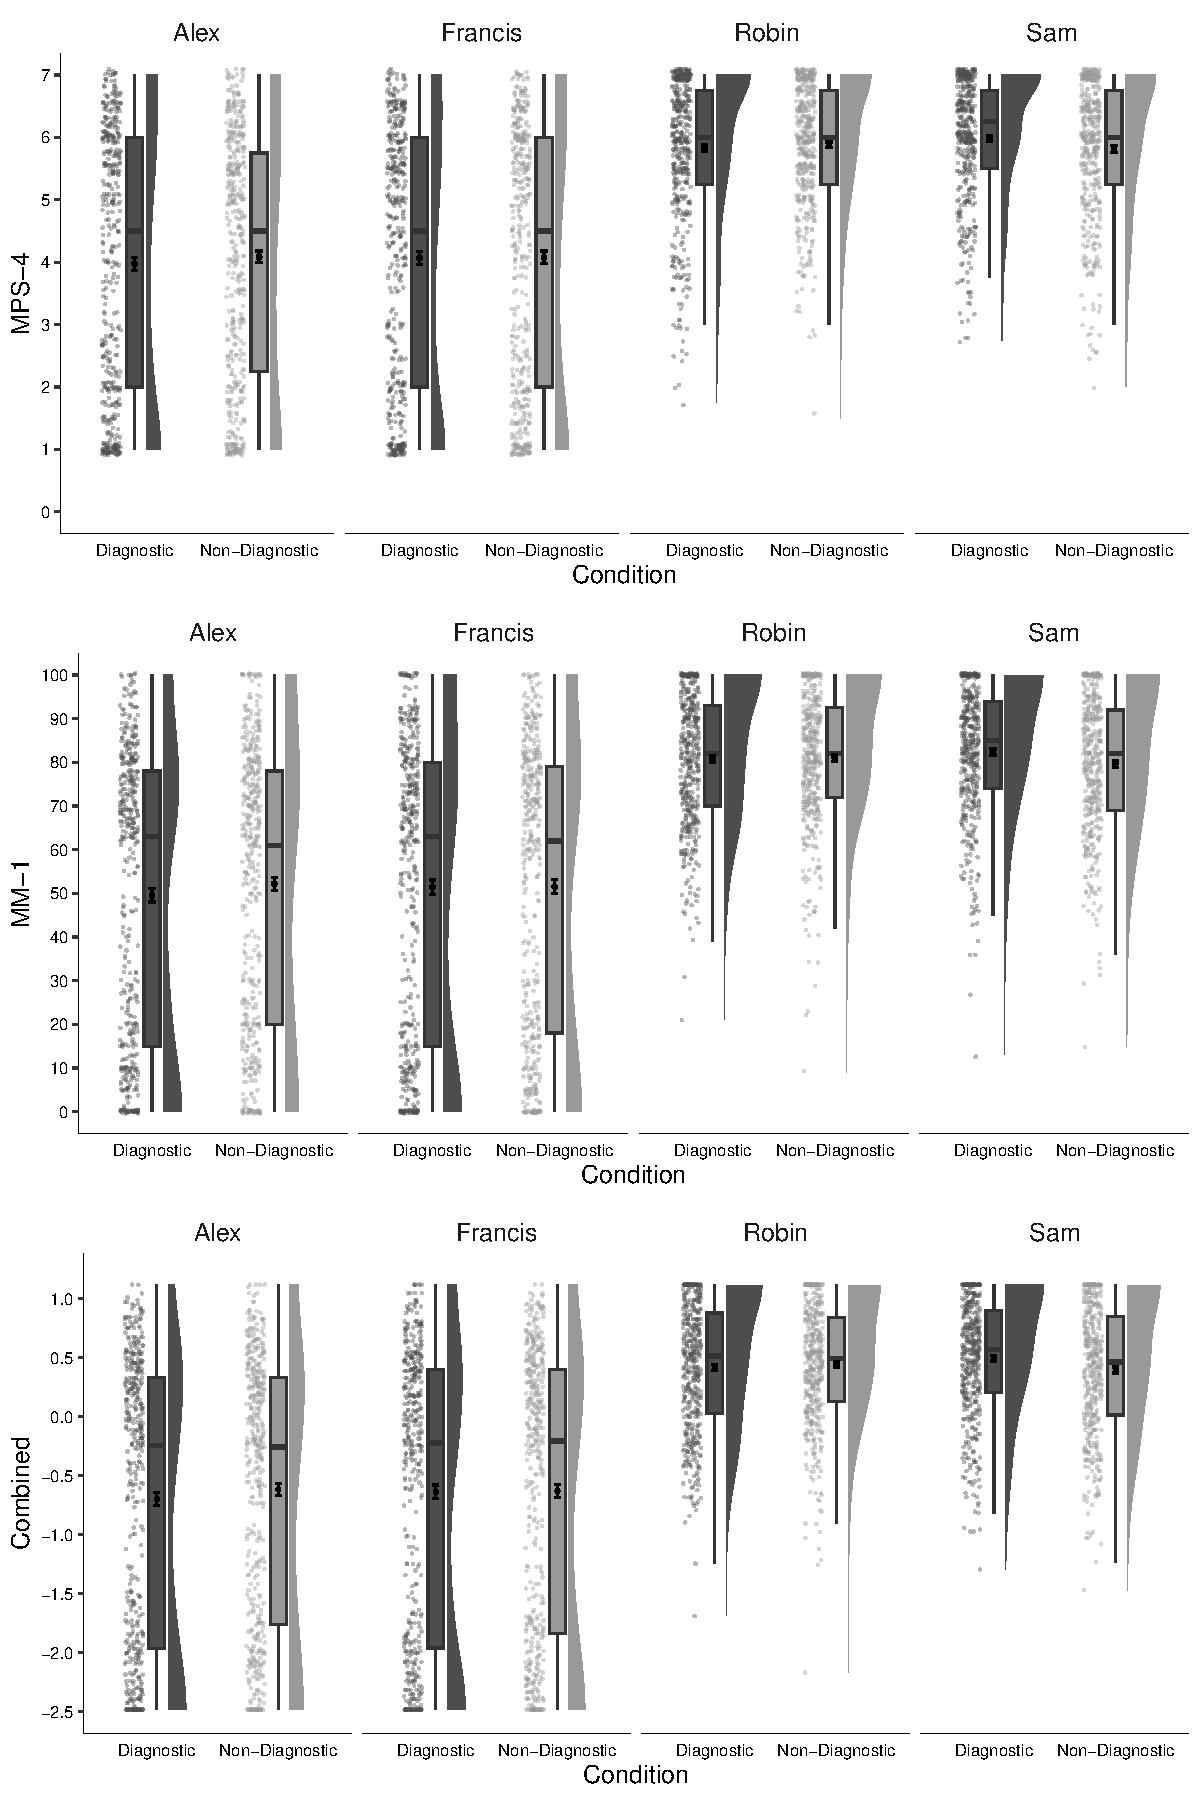
\includegraphics{Supplementary_files/figure-latex/StudyS2AllscenariosPlot-1} \caption{Study 3: Differences in moral perception for each description}\label{fig:StudyS2AllscenariosPlot}
\end{figure}

\subsection{Study S2: Differences between the descriptions}\label{study-s2-differences-between-the-descriptions}

Again, we conducted separate analyses to investigate of condition on responses to each scenario individually. The responses for each scenario across each measure depending on condition are displayed in Figure~\ref{fig:StudyS2AllscenariosPlot}.

For \emph{Sam} (\emph{good}), MPS-4 scores were significantly lower in the non-diagnostic condition (\emph{M} = 5.81, \emph{SD} = 1.09), than in the diagnostic condition (\emph{M} = 5.98, \emph{SD} = 0.97), \emph{t}(859.15) = 2.46, \emph{p} = .014, \emph{d} = 0.17; Similarly, MM-1 ratings were significantly lower in the non-diagnostic condition (\emph{M} = 79.64, \emph{SD} = 15.68), than in the diagnostic condition (\emph{M} = 82.37, \emph{SD} = 14.67), \emph{t}(867.08) = 2.66, \emph{p} = .008, \emph{d} = 0.18. For the combined measure ratings were also lower in the non-diagnostic condition (\emph{M} = 0.39, \emph{SD} = 0.54), than in the diagnostic condition (\emph{M} = 0.50, \emph{SD} = 0.50), \emph{t}(863.14) = 2.85, \emph{p} = .004, \emph{d} = 0.19.

For \emph{Robin} (\emph{good}), MPS-4 scores were not significantly different for the non-diagnostic condition (\emph{M} = 5.88, \emph{SD} = 0.96), than in the diagnostic condition (\emph{M} = 5.83, \emph{SD} = 1.14), \emph{t}(844.53) = -0.77, \emph{p} = .440, \emph{d} = 0.05; MM-1 ratings were similar in the non-diagnostic condition (\emph{M} = 80.92, \emph{SD} = 15.27), and in the diagnostic condition (\emph{M} = 80.70, \emph{SD} = 15.07), \emph{t}(871.98) = -0.22, \emph{p} = .828, \emph{d} = 0.01. For the combined measure ratings were also similar in the non-diagnostic condition (\emph{M} = 0.44, \emph{SD} = 0.51), than in the diagnostic condition (\emph{M} = 0.42, \emph{SD} = 0.54), \emph{t}(867.63) = -0.57, \emph{p} = .569, \emph{d} = 0.04.

For \emph{Alex} (\emph{bad}), MPS-4 scores were not significantly different for the non-diagnostic condition (\emph{M} = 4.08, \emph{SD} = 1.96), than in the diagnostic condition (\emph{M} = 3.97, \emph{SD} = 2.11), \emph{t}(865.81) = -0.80, \emph{p} = .421, \emph{d} = 0.05; MM-1 ratings were similar in the non-diagnostic condition (\emph{M} = 52.19, \emph{SD} = 31.29), and in the diagnostic condition (\emph{M} = 49.58, \emph{SD} = 32.95), \emph{t}(868.76) = -1.20, \emph{p} = .230, \emph{d} = 0.08. For the combined measure ratings were also similar in the non-diagnostic condition (\emph{M} = -0.62, \emph{SD} = 1.11), and in the diagnostic condition (\emph{M} = -0.70, \emph{SD} = 1.19), \emph{t}(867.67) = -1.04, \emph{p} = .301, \emph{d} = 0.07.

For \emph{Francis} (\emph{bad}), MPS-4 scores were not significantly different for the non-diagnostic condition (\emph{M} = 4.08, \emph{SD} = 2.07), than in the diagnostic condition (\emph{M} = 4.07, \emph{SD} = 2.07), \emph{t}(871.94) = -0.09, \emph{p} = .928, \emph{d} = 0.01; MM-1 ratings were not significantly different in the non-diagnostic condition (\emph{M} = 51.56, \emph{SD} = 32.68), than in the diagnostic condition (\emph{M} = 51.42, \emph{SD} = 33.70), \emph{t}(871.59) = -0.06, \emph{p} = .952, \emph{d} = 0.00. For the combined measure ratings were also similar in the non-diagnostic condition (\emph{M} = -0.63, \emph{SD} = 1.18), and in the diagnostic condition (\emph{M} = -0.64, \emph{SD} = 1.20), \emph{t}(871.88) = -0.08, \emph{p} = .939, \emph{d} = 0.01.

\pagebreak

\section{Study S3 - Good and Bad Characters}\label{study-s3---good-and-bad-characters}

The aim of Study S3 was to test for the moral dilution effect in both good and bad characters, while attempting to eliminate the confounding influence of the presence of other descriptions by adopting a between-subjects design.

\subsection{Study S3: Method}\label{study-s3-method}

\subsubsection{Study S3: Participants and design}\label{study-s3-participants-and-design}

Study S3 was a 2 \(\times\) 2 between-subjects factorial design. As in Study 3, the first independent variable was condition with two levels, diagnostic and non-diagnostic. The second independent variable was valence of character description, with two levels morally good and morally bad. We used the same two dependent variables as in previous studies (MPS-4, \(\alpha\) = 0.97, and MM-1).

A total sample of 2389 (1137 female, 1236 male, 5 non-binary, 3 other; 8 prefer not to say, \emph{M}\textsubscript{age} = 38.78, min = 2, max = 1995, \emph{SD} = 42.71) started the survey. Participants were recruited from MTurk and paid \$0.10 for their participation.

Participants who failed both manipulation checks were removed (\emph{n} = 445), leaving a total sample of 1944 participants (960 female, 970 male, 2 other, 2 prefer not to say; \emph{M}\textsubscript{age} = 37.88, min = 2, max = 454, \emph{SD} = 15.49).

\subsubsection{Study S3: Procedure and materials}\label{study-s3-procedure-and-materials}

The materials for Study S3 were the same as those used in Study 3. Participants were randomly presented with a single character description: \emph{Sam}, \emph{Robin} (\emph{good} characters), \emph{Francis} and \emph{Alex} (\emph{bad} characters), and were randomly assigned to the diagnostic condition (containing diagnostic information only), or the non-diagnostic condition (where the character description additionally included non-diagnostic information). Study S3 was not pre-registered however our predictions were the same as those for Study 3.

\subsection{Study S3: Results}\label{study-s3-results}

The means and standard deviations for MPS-4 for each scenario are as follows:
\emph{Sam} (good),
\emph{M}\textsubscript{MPS-4} = 6.15, \emph{SD}\textsubscript{MPS-4} = 0.87,
\emph{Francis} (bad),
\emph{M}\textsubscript{MPS-4} = 3.65, \emph{SD}\textsubscript{MPS-4} = 2.16,
\emph{Alex} (bad),
\emph{M}\textsubscript{MPS-4} = 3.65, \emph{SD}\textsubscript{MPS-4} = 2.09,
\emph{Robin} (good),
\emph{M}\textsubscript{MPS-4} = 6.21, \emph{SD}\textsubscript{MPS-4} = 0.85. There was significant variation depending on the description, \emph{F}(3,1940) = 396.86, \emph{p} \textless{} .001, partial \(\eta\)\textsuperscript{2} = 0.38. Both the \emph{good} characters (\emph{Robin} and \emph{Sam}) were rated significantly more favorably than both the \emph{bad} characters (\emph{Alex} and \emph{Francis}; all \emph{p}s \textless{} .001). There were no differences between \emph{Robin} and \emph{Sam} (\emph{good}: \emph{p} = .932) or between \emph{Alex} and \emph{Francis} (\emph{bad}; \emph{p} \textgreater{} .999).

The means and standard deviations for MM-1 for each scenario are as follows:
\emph{Sam} (good),
\emph{M}\textsubscript{MM-1} = 84.70, \emph{SD}\textsubscript{MM-1} = 15.32;
\emph{Francis} (bad),
\emph{M}\textsubscript{MM-1} = 43.37, \emph{SD}\textsubscript{MM-1} = 34.96;
\emph{Alex} (bad),
\emph{M}\textsubscript{MM-1} = 44.68, \emph{SD}\textsubscript{MM-1} = 34.57;
\emph{Robin} (good),
\emph{M}\textsubscript{MM-1} = 85.33, \emph{SD}\textsubscript{MM-1} = 14.47. There was significant variation depending on the description, \emph{F}(3,1940) = 383.99, \emph{p} \textless{} .001, partial \(\eta\)\textsuperscript{2} = 0.37. Both the \emph{good} characters (\emph{Robin} and \emph{Sam}) were rated significantly more favorably than both the \emph{bad} characters (\emph{Alex} and \emph{Francis}; all \emph{p}s \textless{} .001). There were no differences between \emph{Robin} and \emph{Sam} (\emph{good}: \emph{p} = .982) or between \emph{Alex} and \emph{Francis} (\emph{bad}; (\emph{p} = .872)).

We conducted a 2 \(\times\) 2 between subjects ANOVA to test for an interaction between valence and condition in predicting MPS-4.
Condition significantly influenced responses to the MPS-4,
\emph{F}(1, 1940) = 5.16, \emph{p} = .023;
valence significantly predicted responses,
\emph{F}(1, 1940) = 1,495.09, \emph{p} \textless{} .001;
and there was no significant condition \(\times\) valence interaction,
\emph{F}(1, 1940) = 0.03, \emph{p} = .858.

We conducted a 2 \(\times\) 2 between subjects ANOVA to test for an interaction between valence and condition in predicting responses to MM-1.
Condition significantly influenced responses to MM-1,
\emph{F}(1, 1940) = 9.46, \emph{p} = .002;
valence significantly predicted responses,
\emph{F}(1, 1940) = 580.03, \emph{p} \textless{} .001;
and there was no significant condition \(\times\) valence interaction,
\emph{F}(1, 1940) = 0.32, \emph{p} = .573.

We conducted a 2 \(\times\) 2 between subjects ANOVA to test for an interaction between valence and condition in predicting responses to the combined measure.
Condition significantly influenced responses to the combined measure,
\emph{F}(1, 1940) = 9.46, \emph{p} = .002;
valence significantly predicted responses,
\emph{F}(1, 1940) = 580.03, \emph{p} \textless{} .001;
and there was no significant condition \(\times\) valence interaction,
\emph{F}(1, 1940) = 0.32, \emph{p} = .573.

As in previous studied we conducted separate analyses for the good and bad descriptions.

\begin{figure}[!h]
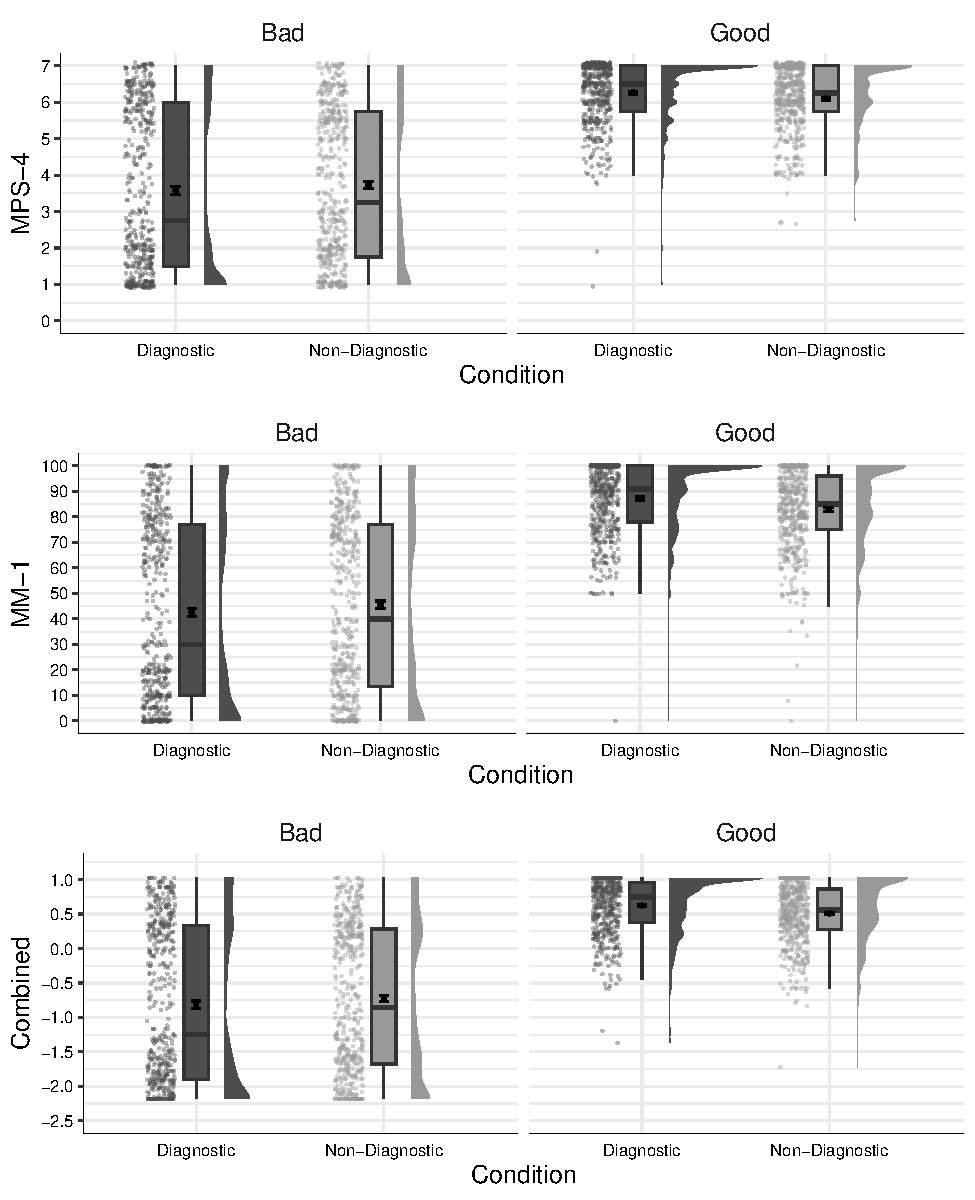
\includegraphics[width=\textwidth,]{Supplementary_files/figure-latex/StudyS3bothconditionplot-1} \caption{Study S3: Differences in moral perception depending on condition}\label{fig:StudyS3bothconditionplot}
\end{figure}

\subsection{\texorpdfstring{Differences in the \emph{Bad} Descriptions}{Differences in the Bad Descriptions}}\label{differences-in-the-bad-descriptions-1}

For the \emph{bad} characters, there was no significant difference in responses to MPS-4 between the diagnostic condition (\emph{M} = 3.57, \emph{SD} = 2.21) and the non-diagnostic condition (\emph{M} = 3.72, \emph{SD} = 2.03) depending on condition, \emph{t}(941.99) = -1.09, \emph{p} = .277, \emph{d} = 0.07.

For the \emph{bad} characters, there was no significant difference in responses to MM-1 between the diagnostic condition (\emph{M} = 34.62, \emph{SD} = 34.25) and the non-diagnostic condition (\emph{M} = 37.04, \emph{SD} = 32.16) depending on condition, \emph{t}(680.45) = -0.96, \emph{p} = .339, \emph{d} = 0.07.

\subsection{\texorpdfstring{Differences in the \emph{Good} Descriptions}{Differences in the Good Descriptions}}\label{differences-in-the-good-descriptions-1}

For the \emph{good} characters, there was no significant difference in responses to MPS-4 between the diagnostic condition (\emph{M} = 6.27, \emph{SD} = 0.84) and the non-diagnostic condition (\emph{M} = 6.09, \emph{SD} = 0.88) depending on condition, \emph{t}(981.90) = 3.21, \emph{p} = .001, \emph{d} = 0.20.

For the \emph{good} characters, there was no significant difference in responses to MPS-4 between the diagnostic condition (\emph{M} = 87.23, \emph{SD} = 13.68) and the non-diagnostic condition (\emph{M} = 82.89, \emph{SD} = 15.70) depending on condition, \emph{t}(972.88) = 4.63, \emph{p} \textless{} .001, \emph{d} = 0.29.

\subsection{Study S3: Differences between the descriptions}\label{study-s3-differences-between-the-descriptions}

Again, we conducted separate analyses to investigate of condition on responses to each scenario individually. The responses for each scenario across each measure depending on condition are displayed in Figure~\ref{fig:StudyS3allscenariosPlot}.

\begin{figure}[!h]
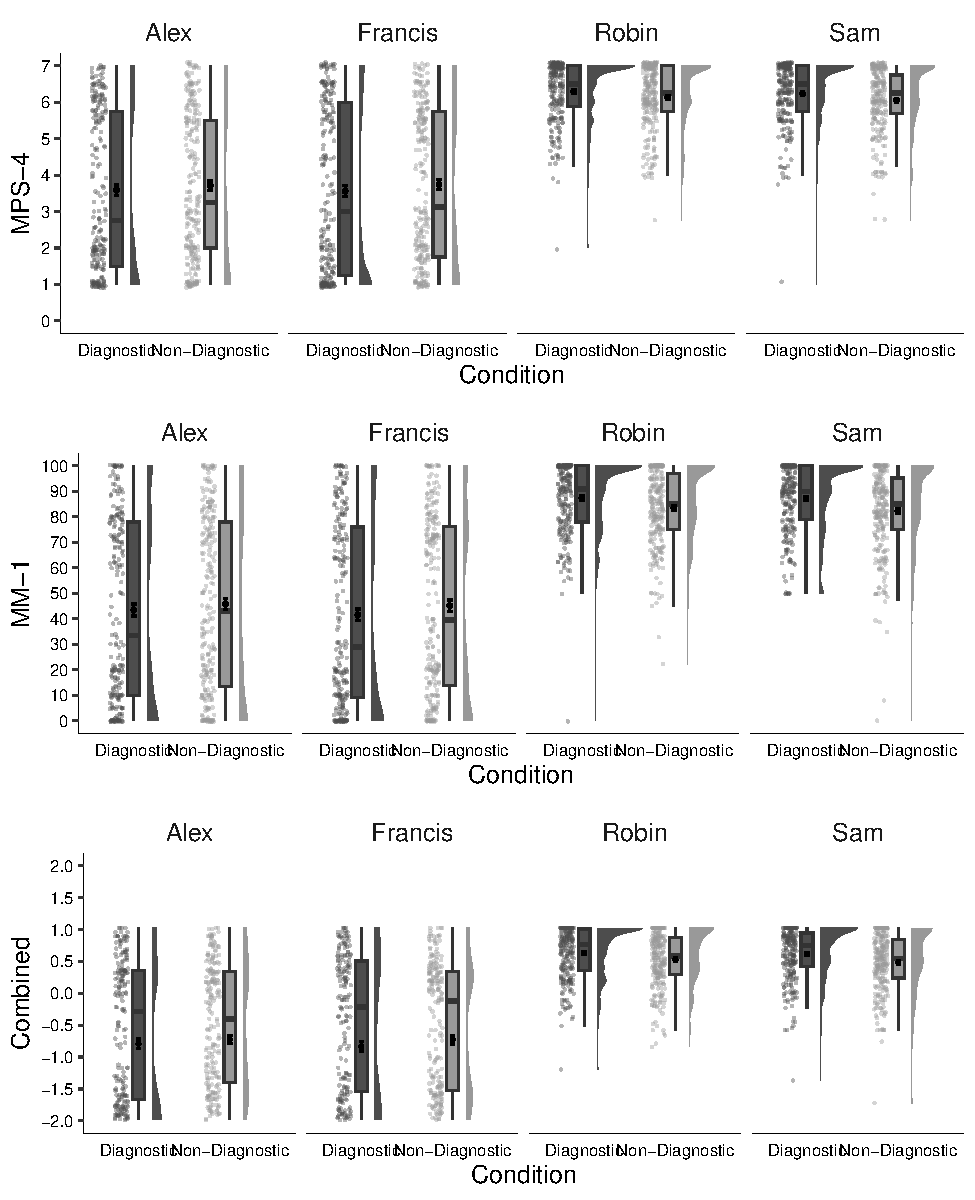
\includegraphics[width=\textwidth,]{Supplementary_files/figure-latex/StudyS3allscenariosPlot-1} \caption{Study S3: Differences in moral perception for each description}\label{fig:StudyS3allscenariosPlot}
\end{figure}

For \emph{Sam}, MPS-4 scores were significantly lower in the non-diagnostic condition (\emph{M} = 6.06, \emph{SD} = 0.89), than in the diagnostic condition (\emph{M} = 6.24, \emph{SD} = 0.85), \emph{t}(488.52) = 2.34, \emph{p} = .020, \emph{d} = 0.21; Similarly, MM-1 ratings were significantly lower in the non-diagnostic condition (\emph{M} = 82.23, \emph{SD} = 16.63), than in the diagnostic condition (\emph{M} = 87.21, \emph{SD} = 13.43), \emph{t}(471.87) = 3.65, \emph{p} \textless{} .001, \emph{d} = 0.33. For the combined measure ratings were also lower in the non-diagnostic condition (\emph{M} = 0.49, \emph{SD} = 0.45), than in the diagnostic condition (\emph{M} = 0.62, \emph{SD} = 0.41), \emph{t}(486.39) = 3.35, \emph{p} \textless{} .001, \emph{d} = 0.30.

For \emph{Robin}, MPS-4 scores were not significantly different for the non-diagnostic condition (\emph{M} = 6.13, \emph{SD} = 0.87), than in the diagnostic condition (\emph{M} = 6.30, \emph{SD} = 0.83), \emph{t}(490.93) = 2.21, \emph{p} = .027, \emph{d} = 0.20; MM-1 ratings were similar in the non-diagnostic condition (\emph{M} = 83.53, \emph{SD} = 14.75), and in the diagnostic condition (\emph{M} = 87.25, \emph{SD} = 13.96), \emph{t}(490.98) = 2.88, \emph{p} = .004, \emph{d} = 0.26. For the combined measure ratings were also similar in the non-diagnostic condition (\emph{M} = 0.53, \emph{SD} = 0.42), than in the diagnostic condition (\emph{M} = 0.63, \emph{SD} = 0.40), \emph{t}(490.92) = 2.82, \emph{p} = .005, \emph{d} = 0.25.

For \emph{Alex}, MPS-4 scores were not significantly different for the non-diagnostic condition (\emph{M} = 3.71, \emph{SD} = 2.02), than in the diagnostic condition (\emph{M} = 3.59, \emph{SD} = 2.16), \emph{t}(465.98) = -0.62, \emph{p} = .534, \emph{d} = 0.06; MM-1 ratings were similar in the non-diagnostic condition (\emph{M} = 45.80, \emph{SD} = 33.76), than in the diagnostic condition (\emph{M} = 43.48, \emph{SD} = 35.46), \emph{t}(468.21) = -0.73, \emph{p} = .465, \emph{d} = 0.07. For the combined measure ratings were also similar in the non-diagnostic condition (\emph{M} = -0.72, \emph{SD} = 1.05), than in the diagnostic condition (\emph{M} = -0.79, \emph{SD} = 1.13), \emph{t}(465.61) = -0.69, \emph{p} = .489, \emph{d} = 0.06.

For \emph{Francis}, MPS-4 scores were not significantly different for the non-diagnostic condition (\emph{M} = 3.74, \emph{SD} = 2.05), than in the diagnostic condition (\emph{M} = 3.56, \emph{SD} = 2.27), \emph{t}(474.15) = -0.91, \emph{p} = .364, \emph{d} = 0.08; MM-1 ratings were not significantly different in the non-diagnostic condition (\emph{M} = 45.16, \emph{SD} = 34.18), than in the diagnostic condition (\emph{M} = 41.55, \emph{SD} = 35.73), \emph{t}(478.97) = -1.13, \emph{p} = .258, \emph{d} = 0.10. For the combined measure ratings were also similar in the non-diagnostic condition (\emph{M} = -0.73, \emph{SD} = 1.07), and in the diagnostic condition (\emph{M} = -0.83, \emph{SD} = 1.16), \emph{t}(476.42) = -1.04, \emph{p} = .297, \emph{d} = 0.10.

\pagebreak

\section*{References}\label{references}
\addcontentsline{toc}{section}{References}

\phantomsection\label{refs}
\begin{CSLReferences}{1}{0}
\bibitem[\citeproctext]{ref-grizzard_validating_2020}
Grizzard, M., Fitzgerald, K., Francemone, C. J., Ahn, C., Huang, J., Walton, J., \ldots{} Eden, A. (2020). Validating the extended character morality questionnaire. \emph{Media Psychology}, \emph{23}(1), 107--130. \url{https://doi.org/10.1080/15213269.2019.1572523}

\bibitem[\citeproctext]{ref-walker_better_2021}
Walker, A. C., Turpin, M. H., Fugelsang, J. A., \& Białek, M. (2021). Better the two devils you know, than the one you don't: {Predictability} influences moral judgments of immoral actors. \emph{Journal of Experimental Social Psychology}, \emph{97}, 104220. \url{https://doi.org/10.1016/j.jesp.2021.104220}

\end{CSLReferences}


\end{document}
